% Options for packages loaded elsewhere
\PassOptionsToPackage{unicode}{hyperref}
\PassOptionsToPackage{hyphens}{url}
\PassOptionsToPackage{dvipsnames,svgnames,x11names}{xcolor}
%
\documentclass[
  letterpaper,
  DIV=11,
  numbers=noendperiod]{scrreprt}

\usepackage{amsmath,amssymb}
\usepackage{iftex}
\ifPDFTeX
  \usepackage[T1]{fontenc}
  \usepackage[utf8]{inputenc}
  \usepackage{textcomp} % provide euro and other symbols
\else % if luatex or xetex
  \usepackage{unicode-math}
  \defaultfontfeatures{Scale=MatchLowercase}
  \defaultfontfeatures[\rmfamily]{Ligatures=TeX,Scale=1}
\fi
\usepackage{lmodern}
\ifPDFTeX\else  
    % xetex/luatex font selection
\fi
% Use upquote if available, for straight quotes in verbatim environments
\IfFileExists{upquote.sty}{\usepackage{upquote}}{}
\IfFileExists{microtype.sty}{% use microtype if available
  \usepackage[]{microtype}
  \UseMicrotypeSet[protrusion]{basicmath} % disable protrusion for tt fonts
}{}
\makeatletter
\@ifundefined{KOMAClassName}{% if non-KOMA class
  \IfFileExists{parskip.sty}{%
    \usepackage{parskip}
  }{% else
    \setlength{\parindent}{0pt}
    \setlength{\parskip}{6pt plus 2pt minus 1pt}}
}{% if KOMA class
  \KOMAoptions{parskip=half}}
\makeatother
\usepackage{xcolor}
\setlength{\emergencystretch}{3em} % prevent overfull lines
\setcounter{secnumdepth}{5}
% Make \paragraph and \subparagraph free-standing
\ifx\paragraph\undefined\else
  \let\oldparagraph\paragraph
  \renewcommand{\paragraph}[1]{\oldparagraph{#1}\mbox{}}
\fi
\ifx\subparagraph\undefined\else
  \let\oldsubparagraph\subparagraph
  \renewcommand{\subparagraph}[1]{\oldsubparagraph{#1}\mbox{}}
\fi

\usepackage{color}
\usepackage{fancyvrb}
\newcommand{\VerbBar}{|}
\newcommand{\VERB}{\Verb[commandchars=\\\{\}]}
\DefineVerbatimEnvironment{Highlighting}{Verbatim}{commandchars=\\\{\}}
% Add ',fontsize=\small' for more characters per line
\usepackage{framed}
\definecolor{shadecolor}{RGB}{241,243,245}
\newenvironment{Shaded}{\begin{snugshade}}{\end{snugshade}}
\newcommand{\AlertTok}[1]{\textcolor[rgb]{0.68,0.00,0.00}{#1}}
\newcommand{\AnnotationTok}[1]{\textcolor[rgb]{0.37,0.37,0.37}{#1}}
\newcommand{\AttributeTok}[1]{\textcolor[rgb]{0.40,0.45,0.13}{#1}}
\newcommand{\BaseNTok}[1]{\textcolor[rgb]{0.68,0.00,0.00}{#1}}
\newcommand{\BuiltInTok}[1]{\textcolor[rgb]{0.00,0.23,0.31}{#1}}
\newcommand{\CharTok}[1]{\textcolor[rgb]{0.13,0.47,0.30}{#1}}
\newcommand{\CommentTok}[1]{\textcolor[rgb]{0.37,0.37,0.37}{#1}}
\newcommand{\CommentVarTok}[1]{\textcolor[rgb]{0.37,0.37,0.37}{\textit{#1}}}
\newcommand{\ConstantTok}[1]{\textcolor[rgb]{0.56,0.35,0.01}{#1}}
\newcommand{\ControlFlowTok}[1]{\textcolor[rgb]{0.00,0.23,0.31}{#1}}
\newcommand{\DataTypeTok}[1]{\textcolor[rgb]{0.68,0.00,0.00}{#1}}
\newcommand{\DecValTok}[1]{\textcolor[rgb]{0.68,0.00,0.00}{#1}}
\newcommand{\DocumentationTok}[1]{\textcolor[rgb]{0.37,0.37,0.37}{\textit{#1}}}
\newcommand{\ErrorTok}[1]{\textcolor[rgb]{0.68,0.00,0.00}{#1}}
\newcommand{\ExtensionTok}[1]{\textcolor[rgb]{0.00,0.23,0.31}{#1}}
\newcommand{\FloatTok}[1]{\textcolor[rgb]{0.68,0.00,0.00}{#1}}
\newcommand{\FunctionTok}[1]{\textcolor[rgb]{0.28,0.35,0.67}{#1}}
\newcommand{\ImportTok}[1]{\textcolor[rgb]{0.00,0.46,0.62}{#1}}
\newcommand{\InformationTok}[1]{\textcolor[rgb]{0.37,0.37,0.37}{#1}}
\newcommand{\KeywordTok}[1]{\textcolor[rgb]{0.00,0.23,0.31}{#1}}
\newcommand{\NormalTok}[1]{\textcolor[rgb]{0.00,0.23,0.31}{#1}}
\newcommand{\OperatorTok}[1]{\textcolor[rgb]{0.37,0.37,0.37}{#1}}
\newcommand{\OtherTok}[1]{\textcolor[rgb]{0.00,0.23,0.31}{#1}}
\newcommand{\PreprocessorTok}[1]{\textcolor[rgb]{0.68,0.00,0.00}{#1}}
\newcommand{\RegionMarkerTok}[1]{\textcolor[rgb]{0.00,0.23,0.31}{#1}}
\newcommand{\SpecialCharTok}[1]{\textcolor[rgb]{0.37,0.37,0.37}{#1}}
\newcommand{\SpecialStringTok}[1]{\textcolor[rgb]{0.13,0.47,0.30}{#1}}
\newcommand{\StringTok}[1]{\textcolor[rgb]{0.13,0.47,0.30}{#1}}
\newcommand{\VariableTok}[1]{\textcolor[rgb]{0.07,0.07,0.07}{#1}}
\newcommand{\VerbatimStringTok}[1]{\textcolor[rgb]{0.13,0.47,0.30}{#1}}
\newcommand{\WarningTok}[1]{\textcolor[rgb]{0.37,0.37,0.37}{\textit{#1}}}

\providecommand{\tightlist}{%
  \setlength{\itemsep}{0pt}\setlength{\parskip}{0pt}}\usepackage{longtable,booktabs,array}
\usepackage{calc} % for calculating minipage widths
% Correct order of tables after \paragraph or \subparagraph
\usepackage{etoolbox}
\makeatletter
\patchcmd\longtable{\par}{\if@noskipsec\mbox{}\fi\par}{}{}
\makeatother
% Allow footnotes in longtable head/foot
\IfFileExists{footnotehyper.sty}{\usepackage{footnotehyper}}{\usepackage{footnote}}
\makesavenoteenv{longtable}
\usepackage{graphicx}
\makeatletter
\def\maxwidth{\ifdim\Gin@nat@width>\linewidth\linewidth\else\Gin@nat@width\fi}
\def\maxheight{\ifdim\Gin@nat@height>\textheight\textheight\else\Gin@nat@height\fi}
\makeatother
% Scale images if necessary, so that they will not overflow the page
% margins by default, and it is still possible to overwrite the defaults
% using explicit options in \includegraphics[width, height, ...]{}
\setkeys{Gin}{width=\maxwidth,height=\maxheight,keepaspectratio}
% Set default figure placement to htbp
\makeatletter
\def\fps@figure{htbp}
\makeatother

\KOMAoption{captions}{tableheading}
\makeatletter
\@ifpackageloaded{tcolorbox}{}{\usepackage[skins,breakable]{tcolorbox}}
\@ifpackageloaded{fontawesome5}{}{\usepackage{fontawesome5}}
\definecolor{quarto-callout-color}{HTML}{909090}
\definecolor{quarto-callout-note-color}{HTML}{0758E5}
\definecolor{quarto-callout-important-color}{HTML}{CC1914}
\definecolor{quarto-callout-warning-color}{HTML}{EB9113}
\definecolor{quarto-callout-tip-color}{HTML}{00A047}
\definecolor{quarto-callout-caution-color}{HTML}{FC5300}
\definecolor{quarto-callout-color-frame}{HTML}{acacac}
\definecolor{quarto-callout-note-color-frame}{HTML}{4582ec}
\definecolor{quarto-callout-important-color-frame}{HTML}{d9534f}
\definecolor{quarto-callout-warning-color-frame}{HTML}{f0ad4e}
\definecolor{quarto-callout-tip-color-frame}{HTML}{02b875}
\definecolor{quarto-callout-caution-color-frame}{HTML}{fd7e14}
\makeatother
\makeatletter
\@ifpackageloaded{bookmark}{}{\usepackage{bookmark}}
\makeatother
\makeatletter
\@ifpackageloaded{caption}{}{\usepackage{caption}}
\AtBeginDocument{%
\ifdefined\contentsname
  \renewcommand*\contentsname{Table of contents}
\else
  \newcommand\contentsname{Table of contents}
\fi
\ifdefined\listfigurename
  \renewcommand*\listfigurename{List of Figures}
\else
  \newcommand\listfigurename{List of Figures}
\fi
\ifdefined\listtablename
  \renewcommand*\listtablename{List of Tables}
\else
  \newcommand\listtablename{List of Tables}
\fi
\ifdefined\figurename
  \renewcommand*\figurename{Figure}
\else
  \newcommand\figurename{Figure}
\fi
\ifdefined\tablename
  \renewcommand*\tablename{Table}
\else
  \newcommand\tablename{Table}
\fi
}
\@ifpackageloaded{float}{}{\usepackage{float}}
\floatstyle{ruled}
\@ifundefined{c@chapter}{\newfloat{codelisting}{h}{lop}}{\newfloat{codelisting}{h}{lop}[chapter]}
\floatname{codelisting}{Listing}
\newcommand*\listoflistings{\listof{codelisting}{List of Listings}}
\makeatother
\makeatletter
\makeatother
\makeatletter
\@ifpackageloaded{caption}{}{\usepackage{caption}}
\@ifpackageloaded{subcaption}{}{\usepackage{subcaption}}
\makeatother
\ifLuaTeX
  \usepackage{selnolig}  % disable illegal ligatures
\fi
\usepackage{bookmark}

\IfFileExists{xurl.sty}{\usepackage{xurl}}{} % add URL line breaks if available
\urlstyle{same} % disable monospaced font for URLs
\hypersetup{
  colorlinks=true,
  linkcolor={blue},
  filecolor={Maroon},
  citecolor={Blue},
  urlcolor={Blue},
  pdfcreator={LaTeX via pandoc}}

\author{}
\date{}

\begin{document}

\renewcommand*\contentsname{Table of contents}
{
\hypersetup{linkcolor=}
\setcounter{tocdepth}{2}
\tableofcontents
}
\bookmarksetup{startatroot}

\chapter*{Welcome to Posit Team User
Training!}\label{welcome-to-posit-team-user-training}
\addcontentsline{toc}{chapter}{Welcome to Posit Team User Training!}

\markboth{Welcome to Posit Team User Training!}{Welcome to Posit Team
User Training!}

This book is a companion to the live Posit Team User training workshop
hosted by Posit.

Posit Team is a bundled offering of Posit's three professional data
science tools: Posit Workbench, Posit Connect, and Posit Workbench.
\textbf{For this book, we consider Posit Team users to be data
scientists that are writing code and developing data products (e.g.,
Shiny applications and Quarto documents)}. For Posit Team
administrators, we'd suggest checking out our
\href{https://solutions.posit.co/admin-training/}{Administrator
Training}.

\section*{Workshop Goal}\label{workshop-goal}
\addcontentsline{toc}{section}{Workshop Goal}

\markright{Workshop Goal}

\begin{tcolorbox}[enhanced jigsaw, toprule=.15mm, title=\textcolor{quarto-callout-note-color}{\faInfo}\hspace{0.5em}{Workshop Goal}, opacitybacktitle=0.6, titlerule=0mm, arc=.35mm, bottomrule=.15mm, rightrule=.15mm, colbacktitle=quarto-callout-note-color!10!white, coltitle=black, colframe=quarto-callout-note-color-frame, left=2mm, opacityback=0, colback=white, breakable, bottomtitle=1mm, toptitle=1mm, leftrule=.75mm]

Provide every participant with a \textbf{foundational knowledge} of
Posit Team through interactive (real) data science workflows.

\end{tcolorbox}

What is considered \emph{foundational knowledge}? For this workshop,
foundational knowledge is the \emph{minimum} Posit Team feature set
and/or workflows that every user should be aware of, including:

\textbf{Posit Workbench}

\begin{itemize}
\item
  Integrated Development Environment (IDE) Options
\item
  Data Access
\item
  Job Launcher
\end{itemize}

\textbf{Posit Connect}

\begin{itemize}
\item
  Publishing Methods
\item
  Content Sharing and Access Control
\item
  Job Scheduling
\item
  Supported Content Types
\item
  Runtime Settings
\end{itemize}

\textbf{Posit Package Manager}

\begin{itemize}
\tightlist
\item
  R/Python Package Access
\end{itemize}

\section*{Agenda}\label{agenda}
\addcontentsline{toc}{section}{Agenda}

\markright{Agenda}

This workshop will loosely follow the model of a typical data science
project as described in \href{https://r4ds.hadley.nz/}{R for Data
Science}:

\begin{figure}

\centering{

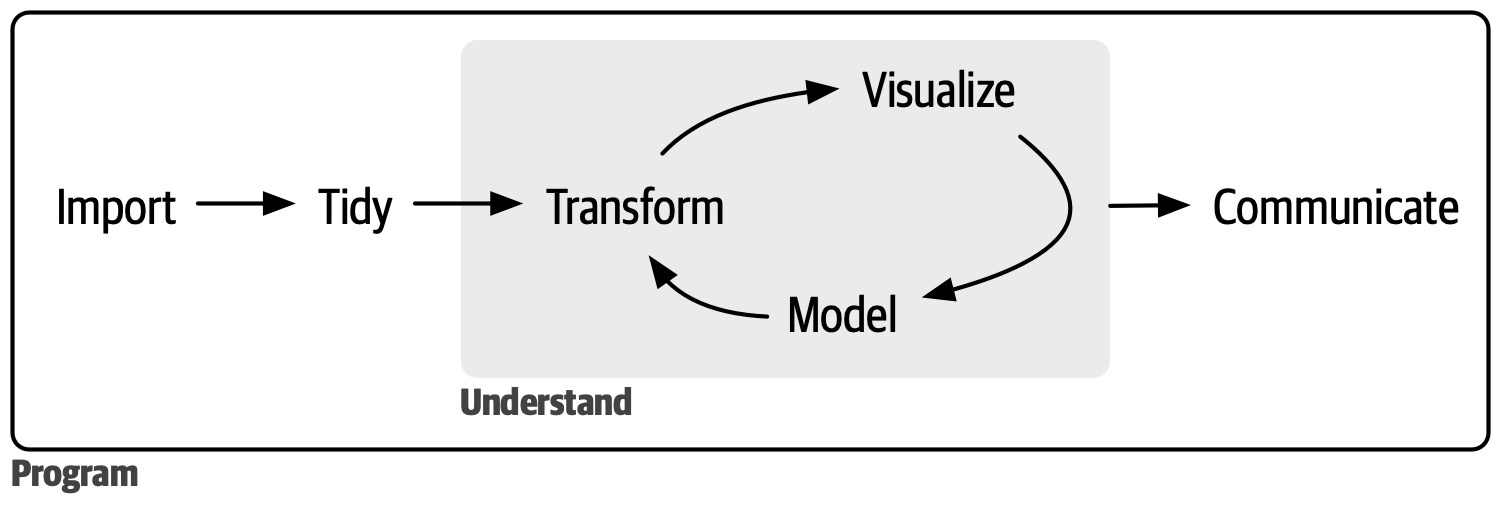
\includegraphics{images/data-science-model.png}

}

\caption{\label{fig-data-science-model}Data science project model}

\end{figure}%

We'll begin with some workshop logistics and an overview of Posit Team.
The remainder of the workshop will follow the above \emph{Data} (focus
on \emph{Import}), \emph{Understand}, and \emph{Communicate} data
science model. A full agenda is listed below:

\begin{itemize}
\item
  Overview and Setup

  \begin{itemize}
  \item
    Accessing the workshop environment
  \item
    Posit Team overview
  \item
    User configuration
  \end{itemize}
\item
  Data

  \begin{itemize}
  \item
    Methods for reading data into Posit Team
  \item
    Posit Professional ODBC Drivers
  \item
    \textbf{Exercise:} Extract-Transform-Load (ETL) workflow
  \end{itemize}
\item
  Understand

  \begin{itemize}
  \item
    Creating a simple model
  \item
    Saving and serving a model
  \item
    \textbf{Exercise:} Create, save, and serve a model using
    \texttt{pins}, \texttt{vetiver}, and FastAPI
  \end{itemize}
\item
  Communicate

  \begin{itemize}
  \item
    Shiny
  \item
    \textbf{Exercise:} Publish a Shiny for Python application to Posit
    Connect
  \item
    \textbf{Exercise:} Publish a Shiny for R application to Posit
    Connect using Git-backed deployment to Posit Connect
  \end{itemize}
\item
  Bonus Content

  \begin{itemize}
  \item
    Connect API
  \item
    \texttt{connectwidgets}
  \item
    Job Launcher in Posit Workbench
  \end{itemize}
\end{itemize}

\part{Overview and Setup}

\chapter{Workshop Access}\label{workshop-access}

\chapter{Posit Team Overview}\label{posit-team-overview}

\begin{figure}

\centering{

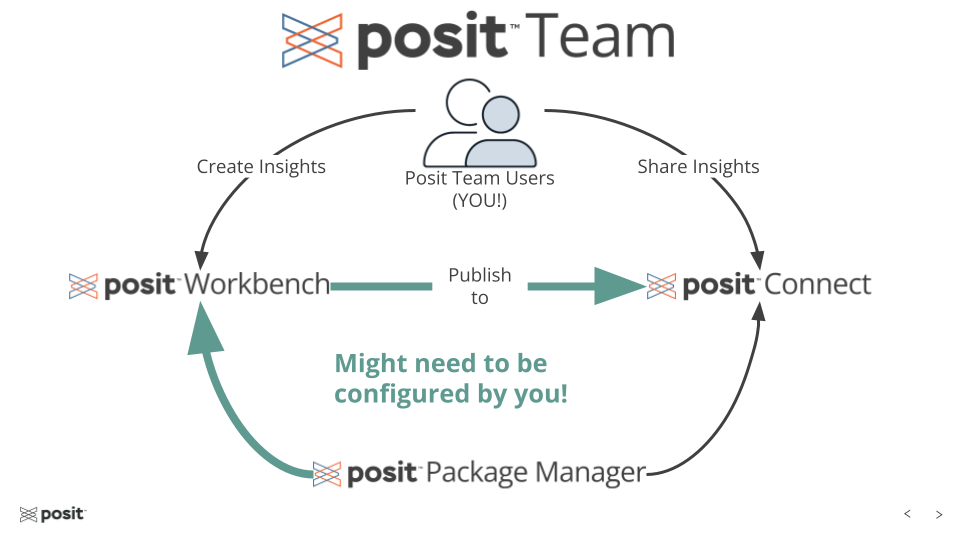
\includegraphics{images/pst-overview.png}

}

\caption{\label{fig-pst-overview}Posit Team Overview}

\end{figure}%

\section{Posit Team}\label{posit-team}

Posit Team is a bundled offering of Posit's three professional data
science tools including Posit Workbench, Posit Connect, and Posit
Package Manager. These tools are designed to fully support end-to-end
data science workflows in both R and Python from code development,
sharing data products, and managing environments.

A quick overview of Posit Team and which development tools, supported
content for hosting, and repository options are shown in
Figure~\ref{fig-pst-features}.

\begin{figure}

\centering{

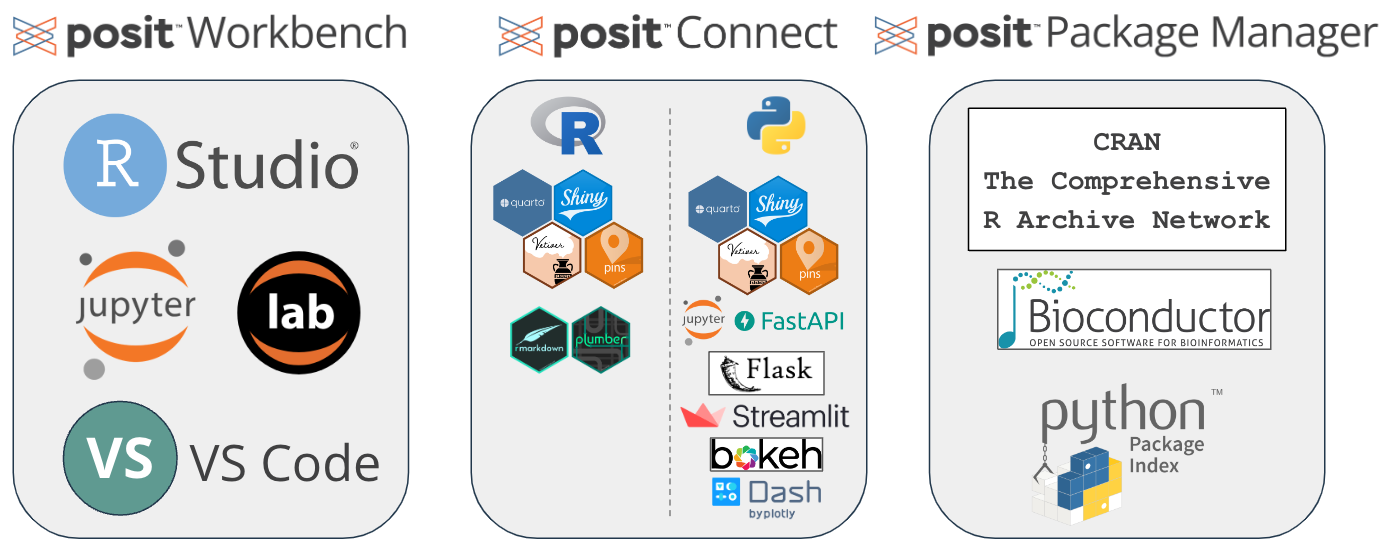
\includegraphics{images/pst-features.png}

}

\caption{\label{fig-pst-features}Posit Team Features}

\end{figure}%

\subsection{Posit Workbench}\label{posit-workbench}

Data scientist leverage Posit Workbench to \emph{create insights}
(Figure~\ref{fig-pst-overview}). As the name implies, Posit Workbench
contains numerous ``tools'' for insight development, including a variety
of integrated development environments (IDEs) to choose from. Currently,
Posit Workbench supports Jupyter Notebook, Jupyter Lab, RStudio Pro and
Visual Studio Code (Figure~\ref{fig-pw-new-session}).

\begin{figure}

\centering{

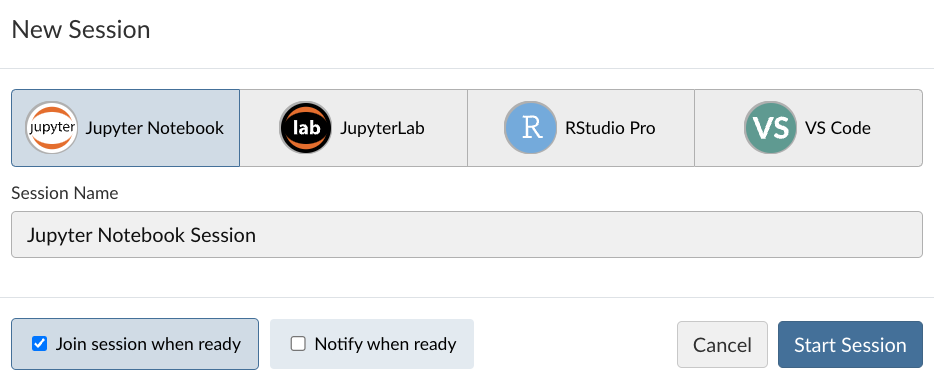
\includegraphics{images/workbench-new-session.png}

}

\caption{\label{fig-pw-new-session}Posit Workbench - New session
options}

\end{figure}%

The IDEs included within Posit Workbench will \emph{look} and
\emph{feel} very similar to the versions that are freely available to
the public. This is by design to ensure users feel at home within Posit
Workbench on day one. There are, however, a few features that you will
only find within Posit Workbench which will be discussed in the next
section.

\subsubsection{Features unique to Posit
Workbench}\label{features-unique-to-posit-workbench}

Many of the \href{https://docs.posit.co/ide/server-pro/}{features} that
make Posit Workbench appealing for data science teams are tailored to
system administrators, IT, and security teams including load balancing,
cluster integration, authentication, session management, and security.
From the users perspective, there are a handful of features that are
worth knowing about which you'll only find within Posit Workbench
including:

\begin{itemize}
\item
  Flexible use of multiple versions of R and Python on the same server.
\item
  Project sharing (RStudio Pro) for easy collaboration within work
  groups.
\item
  Launch long-running scripts (R and Python) in new sessions independent
  of your current working session.
\end{itemize}

\subsection{Posit Connect}\label{posit-connect}

Data scientists leverage Posit Connect to \emph{share insights} with
others (Figure~\ref{fig-pst-overview}). These insights can take many
forms including interactive web applications, static reports,
application programming interfaces (APIs), and more. Once the insights
have been published to Connect (possibly from Posit Workbench), the
publisher has full control over sharing, access, and content execution.

\subsubsection{Publishing Options}\label{publishing-options}

\begin{figure}

\centering{

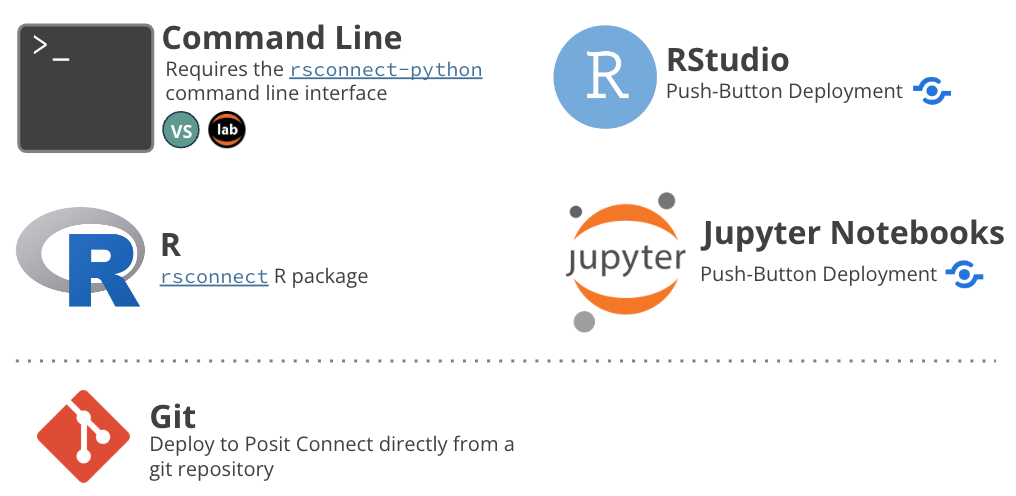
\includegraphics{images/publishing-methods.png}

}

\caption{\label{fig-publishing-methods}Publishing methods}

\end{figure}%

Users have multiple options for publishing content to Posit Connect,
summarized in Figure~\ref{fig-publishing-methods}.

\begin{itemize}
\item
  \textbf{Command Line:} The \texttt{rsconnect-python} package contains
  a command line interface (CLI) tools for publishing content from the
  command line/terminal. During the publishing process, the user's
  environment with automatically be captured and replicated on the Posit
  Connect server. This method is available anywhere you have access to a
  terminal/command line, including Jupyter Lab and VS Code.
\item
  \textbf{Push-Button Deployment}: Available within RStudio and Jupyter
  Notebooks (within Posit Workbench). During the publishing process, the
  user's environment with automatically be captured and replicated on
  the Posit Connect server.
\item
  \textbf{R:} The \texttt{rsconnect} R package makes it easy to publish
  content to Posit Connect from R.
\item
  \textbf{Git}: Deploy content directly from a git repository. In this
  method, the user needs to supply a companion \texttt{manifest.json}
  file which includes information about the environment needed to run
  the content on Posit Connect.
\end{itemize}

\subsection{Posit Package Manager}\label{posit-package-manager}

Data scientists leverage Posit Package Manager to access R and Python
packages from repositories managed and hosted from within your
organization. Often, Posit Package Manager is considered a ``behind the
scenes'' tool, but it's importance should not be underestimated. Users
of Posit Package Manager often find that their package installs and
development environments ``just work'' without any prior configuration.
However, it's still important that users know \emph{how} to install
packages from an instance of Posit Package Manager.

\chapter{User Configuration}\label{user-configuration}

Depending on how your team has installed and configured Posit Team,
there might be no user configurations needed and you can start
developing, installing packages, and publishing immediately!

However, every user should be aware of which configurations are needed
to make Posit Team run like well oiled machine! As show in figure
Figure~\ref{fig-pst-overview}, users should know how to configure Posit
Workbench to use packages from Posit Package Manager and how to
configure a Posit Connect instance for publishing.

\subsection{Configuring your R environment to use Posit Package
Manager}\label{configuring-your-r-environment-to-use-posit-package-manager}

Before making any configurations, you should first check which
repositories you're currently using. Within an active R session, you can
use the \texttt{options} function to explore which repositories
(``repos'') your currently using.

\begin{Shaded}
\begin{Highlighting}[]
\FunctionTok{options}\NormalTok{(}\StringTok{"repos"}\NormalTok{)}
\SpecialCharTok{$}\NormalTok{repos}
\NormalTok{                                         CRAN }
\StringTok{"https://packagemanager.posit.co/cran/latest"}
\end{Highlighting}
\end{Shaded}

In this example, you can see the output is showing
\href{https://packagemanager.posit.co/client/\#/}{Posit's Public Package
Manager} as the default repository for R packages. Specifically, we are
pointing to a \href{https://cran.r-project.org/}{CRAN} repository hosted
within package manager.

To configure R to use Posit Package Manager as it's CRAN repository, set
the \texttt{repos} option to use the repository URL. The
\href{https://docs.posit.co/rspm/user/get-repo-url/}{repository URL} can
be found within the \textbf{SETUP} page within Posit Package Manager.

\begin{Shaded}
\begin{Highlighting}[]
\FunctionTok{options}\NormalTok{(}\AttributeTok{repos =} \FunctionTok{c}\NormalTok{(}\AttributeTok{CRAN =} \StringTok{"https://packagemanager.posit.co/cran/\_\_linux\_\_/centos7/latest"}\NormalTok{))}
\end{Highlighting}
\end{Shaded}

Since this configuration is done within an active R session, you'll need
to repeat these steps anytime you open a new session. Consider adding
this code to your \texttt{.Rprofile} file to maintain the repository
configuration across R sessions.

You can also set the repository URL using the RStudio IDE by navigating
to \textbf{Tools --\textgreater{} Global Options --\textgreater{}
Packages}, and adding the repository URL to the ``Primary CRAN
repository'' text box.

\begin{figure}

\centering{

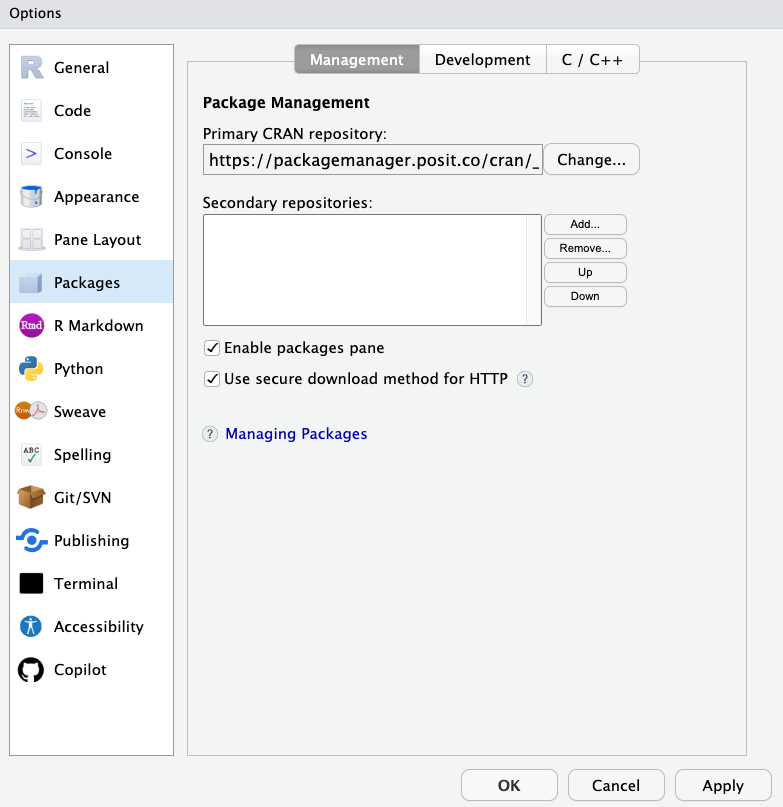
\includegraphics[width=4.01042in,height=\textheight]{images/packages-setting.png}

}

\caption{\label{fig-globaloptions-packages}RStudio Global Options -
Packages}

\end{figure}%

\subsection{Configuring your Python environment to use Posit Package
Manager}\label{configuring-your-python-environment-to-use-posit-package-manager}

Pip is commonly used to install and manage the Python packages in your
environment. To see which repositories pip is currently pointing to, we
can run \texttt{pip\ config\ list} from the command line/terminal:

\begin{Shaded}
\begin{Highlighting}[]
\ExtensionTok{pip}\NormalTok{ config list}
\ExtensionTok{global.index{-}url=}\StringTok{\textquotesingle{}https://packagemanager.posit.co/pypi/latest/simple\textquotesingle{}}
\end{Highlighting}
\end{Shaded}

The \texttt{global.index-url} let's us know which repository pip will
used for python package installation. In this case, it's a mirror of the
\href{https://pypi.org/}{Python Package Index} (PyPI) within Posit
Package Manager.

You can modify the \texttt{global.index-url} setting for all python
projects by running:

\begin{Shaded}
\begin{Highlighting}[]
\ExtensionTok{pip}\NormalTok{ config set global.index{-}url https://packagemanager.posit.co/pypi/latest/simple}
\end{Highlighting}
\end{Shaded}

\section{Configure a Posit Connect instance for
publishing}\label{configure-a-posit-connect-instance-for-publishing}

Publishing your data products to Posit Connect is arguably the most
valuable feature of Posit Team. Configuring a Posit Connect instance
will vary depending on your development environment and publishing
method (see Figure~\ref{fig-publishing-methods}). For this workshop, we
will cover push-button deployment via the RStudio IDE and CLI
publishing. Additional details for configuring a Posit Connect instance
can be found on the
\href{https://docs.posit.co/connect/user/publishing-rstudio/}{Posit
Connect User Guide}.

\subsection{Push Button Deployment
(RStudio)}\label{push-button-deployment-rstudio}

Navigate to \textbf{Tools --\textgreater{} Global Options
--\textgreater{} Publishing.} In some cases, the Posit Connect will
already be configured for you. To add a new Posit Connect instance,
click the \textbf{Connect} button and follow the instructions. The only
thing needed is the Posit Connect URL which can be supplied by your
System Administrator.

\begin{figure}

\centering{

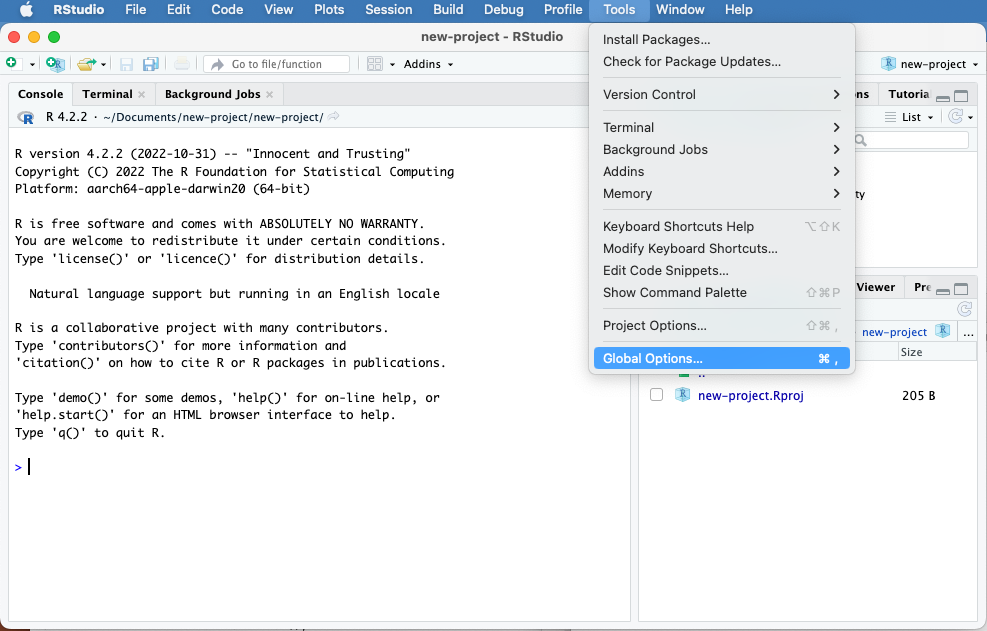
\includegraphics[width=9.79167in,height=\textheight]{images/rstudio-connect1.png}

}

\caption{\label{fig-rstudio-connect1}RStudio - Configure Posit Connect
Instance - Step1}

\end{figure}%

\begin{figure}

\centering{

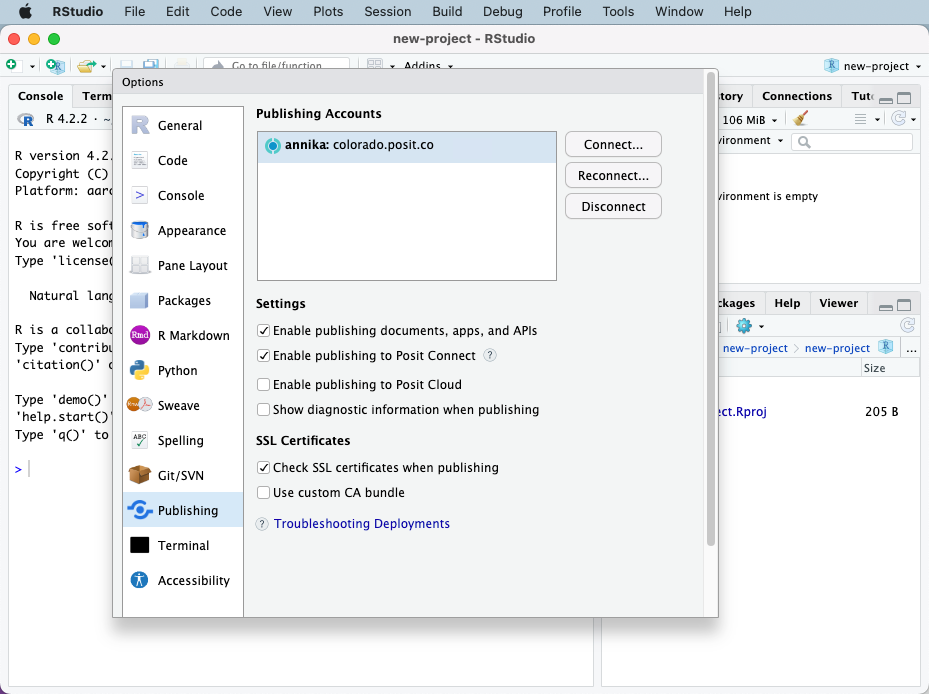
\includegraphics[width=6.15625in,height=\textheight]{images/rstudio-connect2.png}

}

\caption{\label{fig-rstudio-connect2}RStudio - Configure Posit Connect
Instance - Step 2}

\end{figure}%

\section{CLI Publishing}\label{cli-publishing}

To check currenctly connected Posit Connect servers, you can use the
\texttt{rsconnect-python} CLI tool and run the following command from
the terminal/command line:

\begin{Shaded}
\begin{Highlighting}[]
\ExtensionTok{rsconnect}\NormalTok{ add list }
\end{Highlighting}
\end{Shaded}

To add a new Posit Connect instance, you'll need the Posit Connect
server URL as well as an API key (instructions for adding an API can be
found \href{https://docs.posit.co/connect/user/api-keys/}{here}). You
also need to give your Posit Connect instance a name.

\begin{Shaded}
\begin{Highlighting}[]
\ExtensionTok{rsconnect}\NormalTok{ add }\DataTypeTok{\textbackslash{}}
    \AttributeTok{{-}{-}server}\NormalTok{ https://my.connect.server/ }\DataTypeTok{\textbackslash{}}
    \AttributeTok{{-}{-}name}\NormalTok{ myServer }\DataTypeTok{\textbackslash{}}
    \AttributeTok{{-}{-}api{-}key}\NormalTok{ myconnectapikey}
\end{Highlighting}
\end{Shaded}

\part{Data}

\chapter{Data}\label{data-1}

\begin{quote}
{``Data is the new oil!''}

- British mathematician Clive Humbly, 2006
\end{quote}

Data is a precious commodity, playing a key role in informing decisions
and driving insights. Similar to oil, if data is not properly mined,
it's essentially useless. In order for the value of data to be realized,
data science teams need a way to store and access data freely and
readily.

\section{Data Import Options}\label{data-import-options}

Data lives in a variety of locations in a variety of formats, and as
such, there are many options for bringing your data into your
development environment. Below are few common options for accessing your
data:

\begin{figure}

\centering{

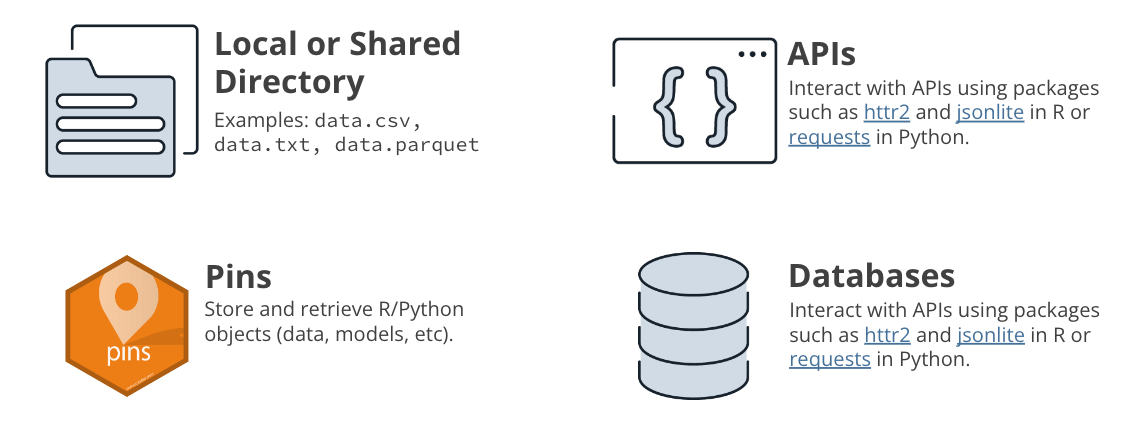
\includegraphics{images/data-import-options.png}

}

\caption{\label{fig-data-import-options}Data import options}

\end{figure}%

Of the four options listed in Figure~\ref{fig-data-import-options},
Databases are the most complex. In the next section, we will give you a
primer on working with databases.

\section{A Primer on Databases}\label{a-primer-on-databases}

Databases are managed by \textbf{D}ata\textbf{B}ase \textbf{M}anagement
\textbf{S}ystems (DBMSs). There exists a growing list of DBMSs for
databases hosted on-prem (client server), in the Cloud, or in-process.
Below are a few common DBMSs:

\begin{figure}

\centering{

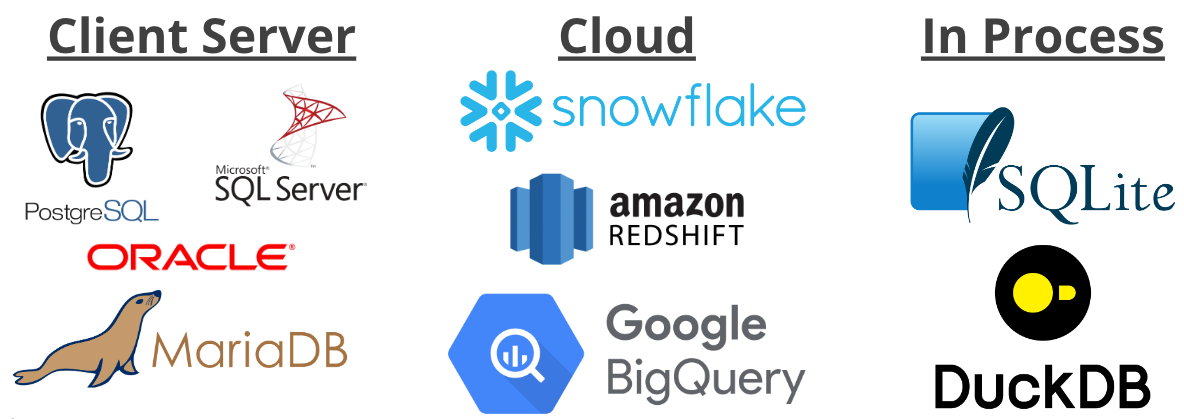
\includegraphics{images/dbms.png}

}

\caption{\label{fig-dbms}Database Management Systems}

\end{figure}%

In R, there exists an \emph{interface} layer between the R programming
language and the DBMS. This is know as the \textbf{D}ata\textbf{B}ase
\textbf{I}nterface (DBI). To make a connection to a DBMS from R, you use
the \texttt{DBI::dbConnect()} function in combination with an R package
tailored for the DBMS you are connecting to. For example, here is some R
code to connect to a PostgreSQL database:

\begin{Shaded}
\begin{Highlighting}[]
\NormalTok{con }\OtherTok{\textless{}{-}}\NormalTok{ DBI}\SpecialCharTok{::}\FunctionTok{dbConnect}\NormalTok{(}
\NormalTok{  RPostgres}\SpecialCharTok{::}\FunctionTok{Postgres}\NormalTok{(), }
  \AttributeTok{hostname =} \StringTok{"databases.mycompany.com"}\NormalTok{, }
  \AttributeTok{port =} \DecValTok{1234}
\NormalTok{)}
\end{Highlighting}
\end{Shaded}

In Python, the database interface layer is an API known as the Python
\textbf{D}ata\textbf{B}ase \textbf{API} (DB-API). Most packages and
modules in Python used to access DBMSs are often designed to be DB-API
compliant including \texttt{sqlite3}, \texttt{psycopg2}, and
\texttt{mysql-connector-python}. For example, here is some Python code
to connect to a SQLite database:

\begin{Shaded}
\begin{Highlighting}[]
\NormalTok{con }\OperatorTok{=}\NormalTok{ sqlite3.}\ExtensionTok{connect}\NormalTok{(}\StringTok{\textquotesingle{}example.db\textquotesingle{}}\NormalTok{)}
\end{Highlighting}
\end{Shaded}

With so many DBMS-specific connectors, it can be overwhelming to
remember which package/function to use. As such, most DBMSs will also
provide a connector known as an \textbf{O}pen \textbf{D}ata\textbf{B}ase
\textbf{C}onnectivity (ODBC) driver. ODBC is a \emph{universal} DBMS
interface, which means the same ODBC functions will work with any
database. For example, here is how to make an ODBC connection to a
PostgreSQL database in R and Python:

\begin{Shaded}
\begin{Highlighting}[]
\CommentTok{\# In R}
\FunctionTok{library}\NormalTok{(DBI)}
\FunctionTok{library}\NormalTok{(odbc)}

\NormalTok{con }\OtherTok{\textless{}{-}}\NormalTok{ DBI}\SpecialCharTok{::}\FunctionTok{dbConnect}\NormalTok{(odbc}\SpecialCharTok{::}\FunctionTok{odbc}\NormalTok{(),}
  \AttributeTok{driver =} \StringTok{"PostgreSQL Driver"}\NormalTok{,}
  \AttributeTok{database =} \StringTok{"test\_db"}\NormalTok{,}
  \AttributeTok{UID    =} \FunctionTok{Sys.getenv}\NormalTok{(}\StringTok{"DB\_USER"}\NormalTok{),}
  \AttributeTok{PWD    =} \FunctionTok{Sys.getenv}\NormalTok{(}\StringTok{"DB\_PASSWORD"}\NormalTok{),}
  \AttributeTok{host =} \StringTok{"localhost"}\NormalTok{,}
  \AttributeTok{port =} \DecValTok{5432}\NormalTok{)}
\end{Highlighting}
\end{Shaded}

\begin{Shaded}
\begin{Highlighting}[]
\CommentTok{\# In Python}
\ImportTok{import}\NormalTok{ pyodbc}

\NormalTok{con }\OperatorTok{=}\NormalTok{ pyodbc.}\ExtensionTok{connect}\NormalTok{(}
\NormalTok{  driver }\OperatorTok{=} \StringTok{\textquotesingle{}PostgreSQL\textquotesingle{}}\NormalTok{,}
\NormalTok{  database }\OperatorTok{=} \StringTok{\textquotesingle{}test\_db\textquotesingle{}}\NormalTok{,}
\NormalTok{  server }\OperatorTok{=} \StringTok{\textquotesingle{}localhost\textquotesingle{}}\NormalTok{,}
\NormalTok{  port }\OperatorTok{=} \DecValTok{5432}\NormalTok{, }
\NormalTok{  uid }\OperatorTok{=}\NormalTok{ os.getenv(}\StringTok{\textquotesingle{}DB\_USER\textquotesingle{}}\NormalTok{),}
\NormalTok{  pwd }\OperatorTok{=}\NormalTok{ os.getenv(}\StringTok{\textquotesingle{}DB\_PASSWORD\textquotesingle{}}\NormalTok{)}
\NormalTok{)}
\end{Highlighting}
\end{Shaded}

\section{Posit's Professional ODBC
Drivers}\label{posits-professional-odbc-drivers}

Not all DBMSs will provide an ODBC Driver. This can be a major blocker
for users attempting to import data into their development environment.
To overcome this limitation, Posit has created custom ODBC drivers that
work with many of the popular DBMSs used today, including:

\begin{figure}

\centering{

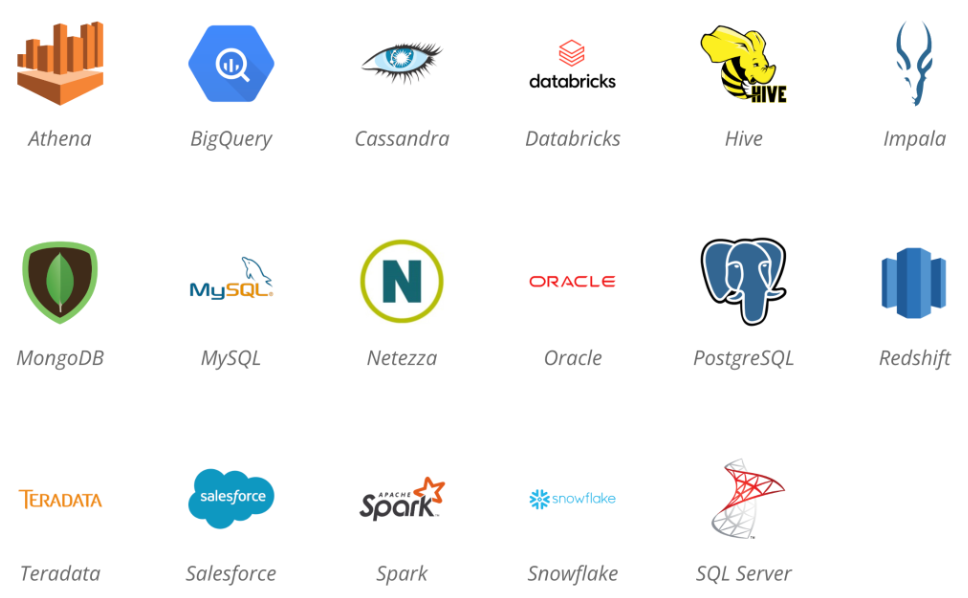
\includegraphics{images/posit-odbc-drivers.png}

}

\caption{\label{fig-posit-odbc-drivers}Posit's Professional ODBC
Drivers}

\end{figure}%

Make sure to speak with your Posit Team system administrator if you
currently use any of the above databases.

\chapter{Exercise: ETL}\label{exercise-etl}

\begin{figure}

\centering{

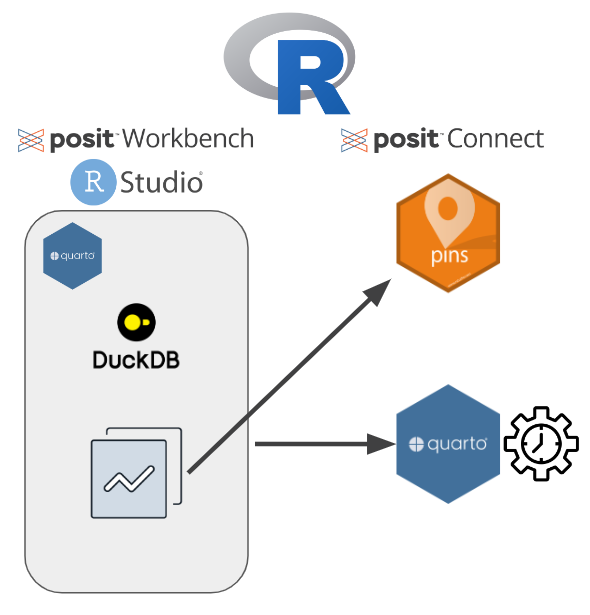
\includegraphics[width=3.85417in,height=\textheight]{images/exercise-etl.png}

}

\caption{\label{fig-etl-workflow}ETL Workflow}

\end{figure}%

A common data science workflow entails \textbf{E}xtracting data,
\textbf{T}ransforming it, and then \textbf{L}oading (ETL) it to a
location to be shared with others or consumed by other content. In this
exercise, you will get practice creating an ETL workflow within Posit
Team. You will also leverage the job scheduling feature in Posit Connect
to ensure the data remains updated automatically.

The data for this exercise is ``real'' data regarding cases of COVID19
in the United States from 2020 to 2023. While this is a relatively small
dataset, the ETL workflow (as shown in Figure~\ref{fig-etl-workflow}) is
designed to work with data of all sizes! Here is a preview of the COVID
dataset with an explanation of the various columns:

\begin{verbatim}
# A tibble: 66,100 x 4
   province_state date       state_count new_cases
   <chr>          <date>           <dbl>     <dbl>
 1 Alabama        2020-01-23           0         0
 2 Alabama        2020-01-24           0         0
 3 Alabama        2020-01-25           0         0
 4 Alabama        2020-01-26           0         0
 5 Alabama        2020-01-27           0         0
 6 Alabama        2020-01-28           0         0
 7 Alabama        2020-01-29           0         0
 8 Alabama        2020-01-30           0         0
 9 Alabama        2020-01-31           0         0
10 Alabama        2020-02-01           0         0
# i 66,090 more rows
\end{verbatim}

\texttt{province\_state}: State or province in the United States of
America.

\texttt{date}: Date of reporting.

\texttt{state\_count}: Total number of confirmed COVID cases in state as
of \texttt{Date}.

\texttt{new\_cases}: Number of new confirmed COVID cases on
\texttt{Date}.

\section{Step 1 - Extract Data from
DuckDB}\label{step-1---extract-data-from-duckdb}

The workshop environment comes with a DuckDB, which can be be found
here: \texttt{duckdb/database/demo-datasets.db}. Within the DuckDB
database is the COVID dataset described in
\textbf{?@sec-etl-background}. The first step is to make a connection to
the DuckDB and read in the COVID data using R.

All of this R code should be added to a
\href{https://quarto.org/}{Quarto} document within the RStudio IDE on
Posit Workbench.

\subsection{Load Necessary Packages}\label{load-necessary-packages}

\begin{Shaded}
\begin{Highlighting}[]
\FunctionTok{library}\NormalTok{(DBI)}
\FunctionTok{library}\NormalTok{(dplyr)}
\FunctionTok{library}\NormalTok{(pins)}
\FunctionTok{library}\NormalTok{(duckdb)}
\FunctionTok{library}\NormalTok{(dbplyr)}
\end{Highlighting}
\end{Shaded}

\subsection{Connect to DuckDB}\label{connect-to-duckdb}

For this connection, we are using the \texttt{DBI} package in
combination with the \texttt{duckDB} package.

\begin{Shaded}
\begin{Highlighting}[]
\NormalTok{con }\OtherTok{\textless{}{-}}\NormalTok{ DBI}\SpecialCharTok{::}\FunctionTok{dbConnect}\NormalTok{(duckdb}\SpecialCharTok{::}\FunctionTok{duckdb}\NormalTok{(), }\AttributeTok{dbdir =} \StringTok{"/data/duckdb/database/demo{-}datasets.db"}\NormalTok{)}
\end{Highlighting}
\end{Shaded}

After the connection (\texttt{con}) has been made, you can explore the
various dataset contained within the DuckDB by running:

\begin{Shaded}
\begin{Highlighting}[]
\FunctionTok{dbListTables}\NormalTok{(con)}
\end{Highlighting}
\end{Shaded}

\subsection{Extract/Transform Covid
Data}\label{extracttransform-covid-data}

Let's use the \texttt{dplyr::tbl()} function to extract the Covid data
from the DuckDB connection. The \texttt{tbl()} makes a ``pointer'' to
the COVID data within the DuckDB. To pull the data into our active R
session and store it in memory, we need to use the
\texttt{dplyr::collect()} function:

\begin{Shaded}
\begin{Highlighting}[]
\NormalTok{covid }\OtherTok{\textless{}{-}} \FunctionTok{tbl}\NormalTok{(con, }\StringTok{"covid"}\NormalTok{) }\SpecialCharTok{|\textgreater{}} 
  \CommentTok{\# Read into memory}
  \FunctionTok{collect}\NormalTok{()}
\end{Highlighting}
\end{Shaded}

In order to save compute resources in your R session, it's suggested to
do any type of cleaning and filtering of the data before calling the
\texttt{collect()} function. Therefore, let's amend the previous code
and insert a \emph{transformation} step before the \texttt{collect()}
function to filter our data for a specific state/province. Feel free to
substitute ``Maryland'' in the code below for another state/province:

\begin{Shaded}
\begin{Highlighting}[]
\NormalTok{covid }\OtherTok{\textless{}{-}} \FunctionTok{tbl}\NormalTok{(con, }\StringTok{"covid"}\NormalTok{) }\SpecialCharTok{|\textgreater{}}
  \CommentTok{\# Filter for a state/provice}
  \FunctionTok{filter}\NormalTok{(province\_state }\SpecialCharTok{==} \StringTok{"Maryland"}\NormalTok{) }\SpecialCharTok{|\textgreater{}}
  \CommentTok{\# Read into memory}
  \FunctionTok{collect}\NormalTok{()}
\end{Highlighting}
\end{Shaded}

\section{Step 2 - Load Data to Posit
Connect}\label{step-2---load-data-to-posit-connect}

Now that the data has been transformed (filtered for a specific
state/province), it's time to \emph{load} the data so that other
users/content can access it. For this exercise, we are going to use the
popular \texttt{pins} package to load the data to Posit Connect.

Pinning an object to Posit Connect is a two step process. The first step
is to define Posit Connect as our pinning \emph{board}:

\begin{Shaded}
\begin{Highlighting}[]
\NormalTok{board }\OtherTok{\textless{}{-}}\NormalTok{ pins}\SpecialCharTok{::}\FunctionTok{board\_connect}\NormalTok{()}
\end{Highlighting}
\end{Shaded}

For this workshop, the \texttt{board\_connect()} function should work
without supplying any arguments. When running this command in your own
environment, you may need to do some configuration which is described
\href{https://pins.rstudio.com/reference/board_connect.html}{here}.

The second step is to write the data to Posit Connect as a pin. Before
running the code below, take note of what your username is on the Posit
Connect server. In this example, I'm using the placeholder name of
\texttt{publisher1}, but be sure to replace this with \textbf{your}
username!

\begin{Shaded}
\begin{Highlighting}[]
\NormalTok{pins}\SpecialCharTok{::}\FunctionTok{pin\_write}\NormalTok{(}\AttributeTok{board =}\NormalTok{ board, }\AttributeTok{x =}\NormalTok{ covid, }\AttributeTok{name =} \StringTok{"publisher1/covid\_data"}\NormalTok{, }\AttributeTok{type =} \StringTok{"csv"}\NormalTok{)}
\end{Highlighting}
\end{Shaded}

\section{Step 3 - Publish Workflow and
Automate}\label{step-3---publish-workflow-and-automate}

Although the COVID dataset is static, from early 2020 to mid 2023, it
was being updated daily. If the data changes, you'll need to re-run the
ETL workflow described above to ensure the pinned dataset reflects the
latest data. This is a manual process that we can automate with the help
of Posit Team!

First, click the blue deployment button at the top of the RStudio IDE:

\begin{figure}

\centering{

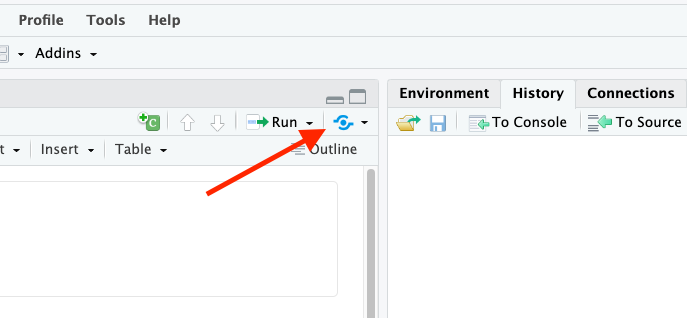
\includegraphics[width=7.14583in,height=\textheight]{images/deployment-button.png}

}

\caption{\label{fig-deployment-button}RStudio - Deployment Button}

\end{figure}%

In the subsequent pop-up window, select \textbf{Posit Connect.}
Importantly, to re-run the quarto document on the Connect server, we
need to \textbf{publish document with source code}:

\begin{figure}

\centering{

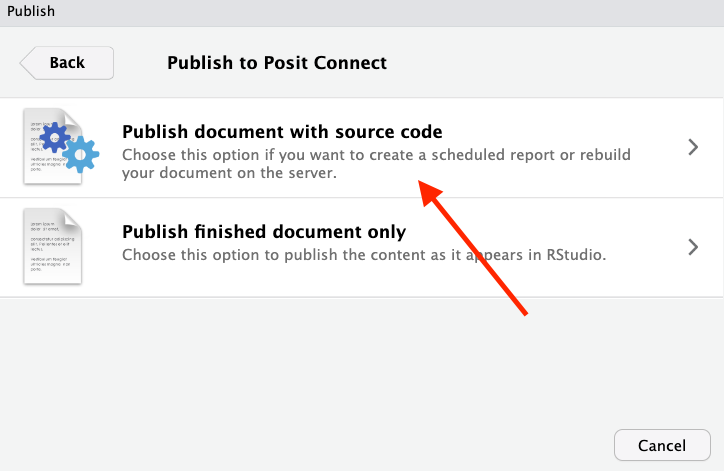
\includegraphics{images/with-source-code.png}

}

\caption{\label{fig-with-source-code}RStudio - Publish Options}

\end{figure}%

The last step is to define the files you want to send to Connect, the
Connect instance you want to publish to, and the title of the content.
If everything looks good, go ahead and click \textbf{Publish}!

\begin{figure}

\centering{

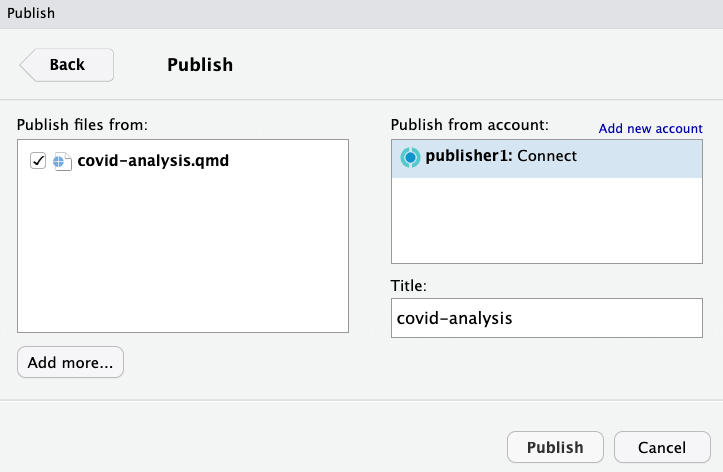
\includegraphics{images/rstudio-publish.png}

}

\caption{\label{fig-rstudio-publish}RStudio - Publish to Posit Connect}

\end{figure}%

Once hosted on Connect, let's set the Quarto document to re-run on a
daily basis. We accomplish this by selecting the \emph{Schedule} tab at
the top. In the below configuration, the Quarto document will run every
day at 9:48 am (America - New York time) and will ensure the pinned
dataset is always up-to-date!

\begin{figure}

\centering{

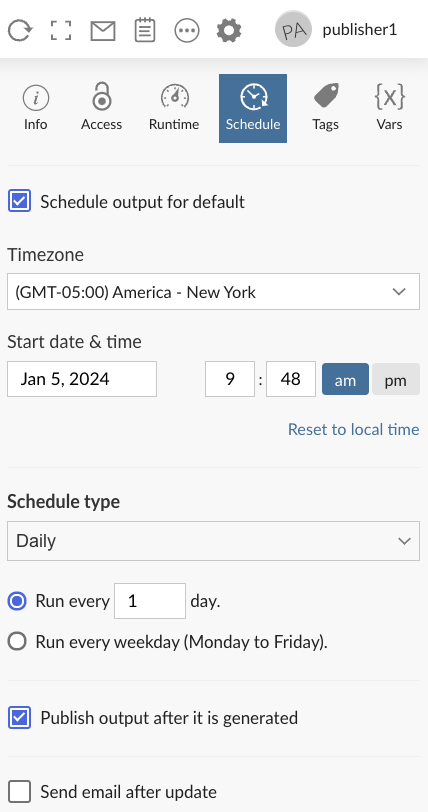
\includegraphics{images/schedule.png}

}

\caption{\label{fig-schedule}Job Scheduling on Posit Connect}

\end{figure}%

You'll also notice at the bottom we have two options to publish the
output after it is generated and send email after update. The first
option ensure that the content on Posit Connect is updated after it's
scheduled to run. This is important if your content has any plots or
tables that need to be updated. The second option allows you to send an
email to users with a direct link to the content on Posit Connect. This
is a great option to deliver insights for those that love to live in
their email inbox 😁.

\part{Understand}

\chapter{Modeling with Posit Team}\label{modeling-with-posit-team}

Many data science workflows culminate in a deliverable. This could be a
single plot or table, a detailed dashboard, or a interactive web
application. Deliverables must tell a story, and the only way to tell a
good story is to \textbf{understand} the underlying data.

Machine Learning (ML) is an exciting and ever-evolving facet of data
science, offering a valuable means to extract insights from your dataset
that may not be readily apparent through basic plots and tables. While
generating models can pose certain challenges, the greater challenge
often lies in determining the methods to save, distribute, and serve
your model so that others can interact with it. In this chapter, we'll
discuss how Posit Team can be used to support the entire ML life cycle,
from creation to delivery!

\section{The Machine Learning Life
Cycle}\label{the-machine-learning-life-cycle}

\begin{figure}

\centering{

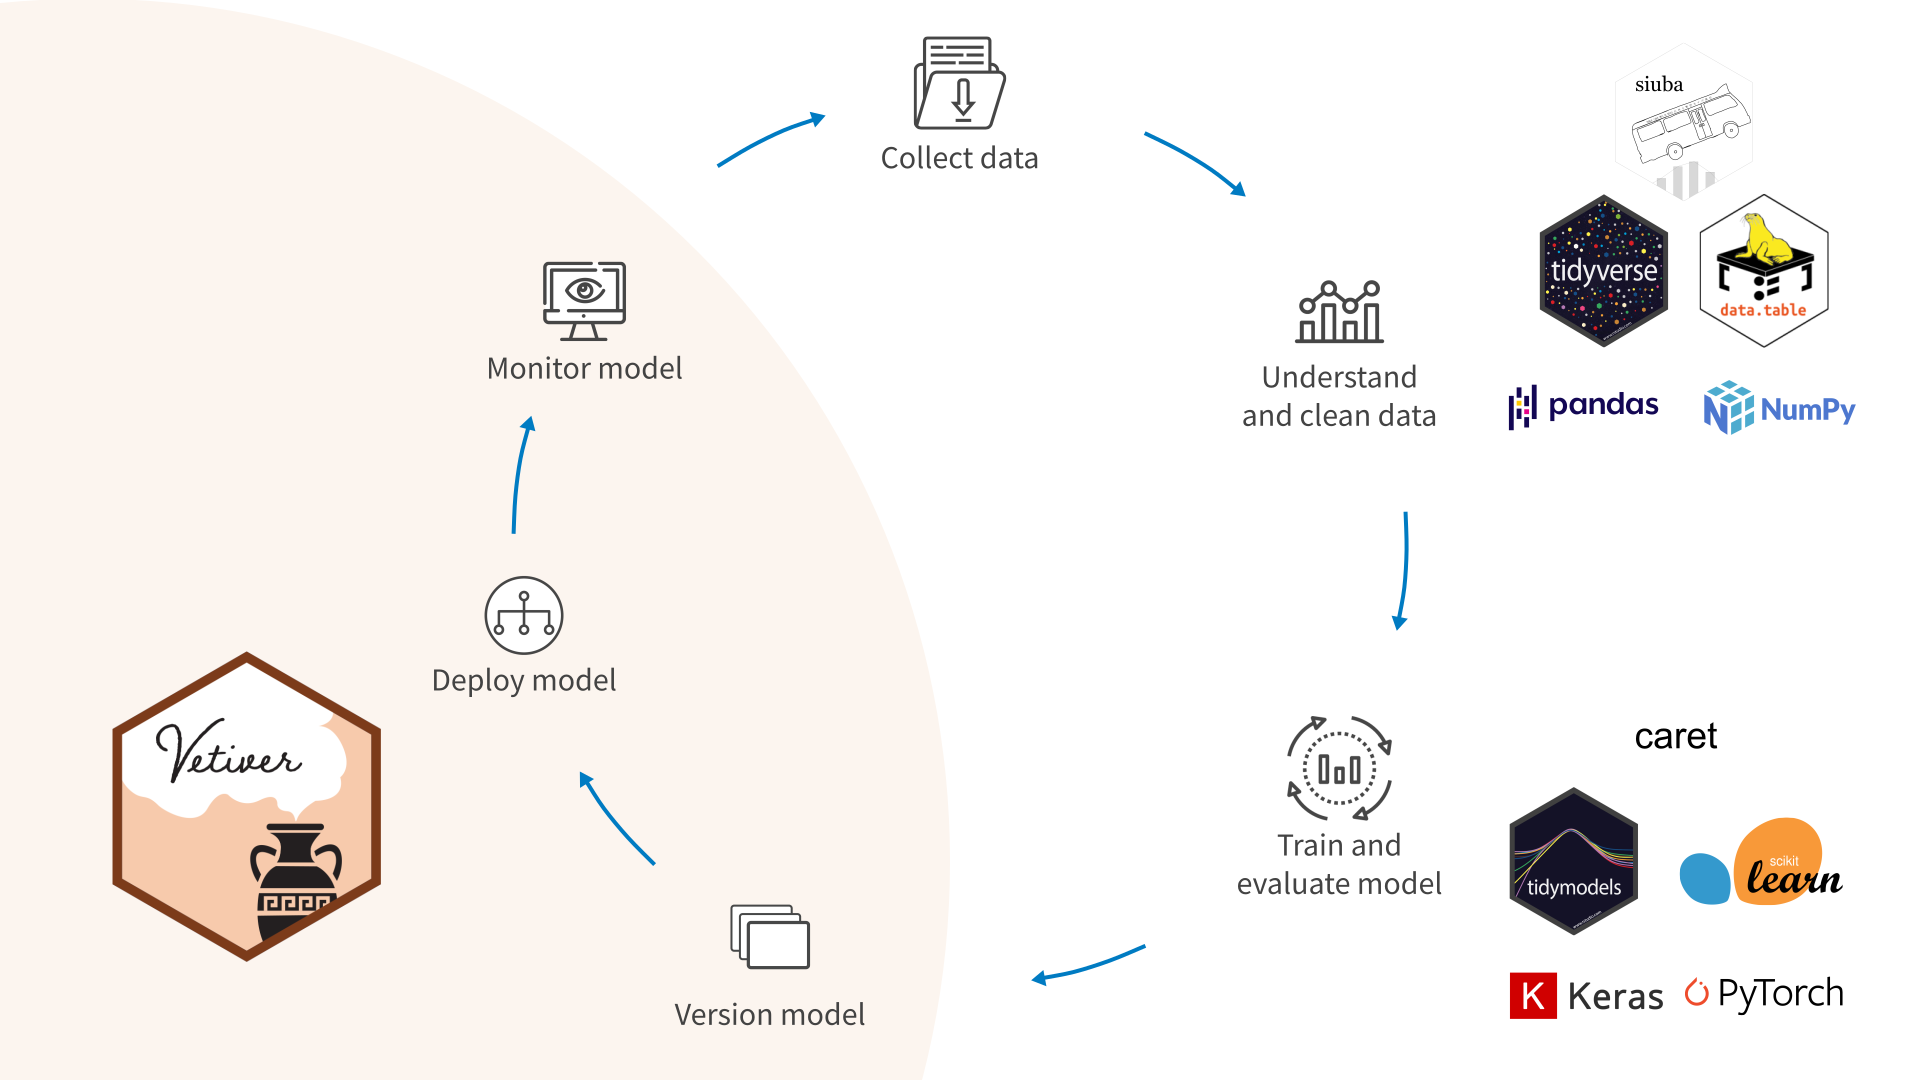
\includegraphics{images/ml_ops_cycle.png}

}

\caption{\label{fig-ml-lifecycle}Machine Learning Life Cycle}

\end{figure}%

As seen in Figure~\ref{fig-ml-lifecycle}, all models start with data
(very top of the cycle). The next step is to prepare the data for
modeling, which requires cleaning and transforming to ensure the data is
in a format that is usable for machine learning. Which tool(s) you use
to create an ML model is completely up to you, but here's a short list
of common R/Python tools:

\begin{longtable}[]{@{}ll@{}}
\caption{Packages, Libraries, and Frameworks for ML Model
Creation}\tabularnewline
\toprule\noalign{}
R & Python \\
\midrule\noalign{}
\endfirsthead
\toprule\noalign{}
R & Python \\
\midrule\noalign{}
\endhead
\bottomrule\noalign{}
\endlastfoot
\texttt{tidymodels} & SciKit-Learn \\
\texttt{caret} & Keras \\
& PyTorch \\
& TensorFlow \\
\end{longtable}

Rarely is the creation of a model a one time event. As data changes and
the ML tools evolve, models will need to be updated and subsequently
deployed into production. It's also important that the deployed model
demonstrates high performance compared to prior versions and other
models.

\section{\texorpdfstring{MLOps with
\texttt{vetiver}}{MLOps with vetiver}}\label{mlops-with-vetiver}

Given the iterative nature of the ML life cycle, there exists tools
explicitly designed to assist with the deployment and maintenance
(i.e.~``operations'') of ML models. This practice is known as
\textbf{M}achine \textbf{L}earning \textbf{O}perations, or
\textbf{MLOps}. Posit has created a MLOps framework for both R and
Python known as \href{https://vetiver.rstudio.com/}{\texttt{vetiver}}.
\texttt{vetiver} was designed to fill the tool gap in the ML life cycle
around versioning, deploying, and monitoring model performance.

\subsection{\texorpdfstring{\texttt{vetiver} workflow with Posit
Team}{vetiver workflow with Posit Team}}\label{vetiver-workflow-with-posit-team}

\includegraphics[width=7.85in,height=0.71in]{modeling_files/figure-latex/mermaid-figure-1.png}

A typical \texttt{vetiver} workflow within Posit Team, depicted in the
flow diagram above, consists of converting a model to a \emph{vetiver
model}, saving it to Posit Connect as a \texttt{pin}, and then serving
it as an API. This workflow is shown below in both Python and R. Be sure
to substitute ``your\_name'' with your Posit Connect username:

\section{Python}

\begin{Shaded}
\begin{Highlighting}[]
\ImportTok{import}\NormalTok{ pins}
\ImportTok{from}\NormalTok{ vetiver }\ImportTok{import}\NormalTok{ VetiverModel}
\ImportTok{from}\NormalTok{ vetiver.data }\ImportTok{import}\NormalTok{ mtcars}
\ImportTok{from}\NormalTok{ sklearn.linear\_model }\ImportTok{import}\NormalTok{ LinearRegression}

\CommentTok{\# Create Model}
\NormalTok{model }\OperatorTok{=}\NormalTok{ LinearRegression().fit(mtcars.drop(columns}\OperatorTok{=}\StringTok{"mpg"}\NormalTok{), mtcars[}\StringTok{"mpg"}\NormalTok{])}

\CommentTok{\# Create Vetiver Model}
\NormalTok{v }\OperatorTok{=}\NormalTok{ VetiverModel(model, model\_name }\OperatorTok{=} \StringTok{"your\_name/cars\_linear"}\NormalTok{, }
\NormalTok{                 prototype\_data }\OperatorTok{=}\NormalTok{ mtcars.drop(columns}\OperatorTok{=}\StringTok{"mpg"}\NormalTok{))}

\CommentTok{\# Save Model as pin}
\NormalTok{board }\OperatorTok{=}\NormalTok{ pins.board\_connect(allow\_pickle\_read }\OperatorTok{=} \VariableTok{True}\NormalTok{)}
\NormalTok{vetiver\_pin\_write(board, v)}
\end{Highlighting}
\end{Shaded}

\section{R}

\begin{Shaded}
\begin{Highlighting}[]
\FunctionTok{library}\NormalTok{(vetiver)}
\FunctionTok{library}\NormalTok{(pins)}

\CommentTok{\# Create Model}
\NormalTok{cars\_lm }\OtherTok{\textless{}{-}} \FunctionTok{lm}\NormalTok{(mpg }\SpecialCharTok{\textasciitilde{}}\NormalTok{ ., }\AttributeTok{data =}\NormalTok{ mtcars)}

\CommentTok{\# Create Vetiver Model}
\NormalTok{v }\OtherTok{\textless{}{-}} \FunctionTok{vetiver\_model}\NormalTok{(cars\_lm, }\StringTok{"your\_name/cars\_linear"}\NormalTok{)}

\CommentTok{\# Save Model as pin}
\NormalTok{board }\OtherTok{\textless{}{-}} \FunctionTok{board\_connect}\NormalTok{()}
\FunctionTok{vetiver\_pin\_write}\NormalTok{(board, v)}
\end{Highlighting}
\end{Shaded}

Now that we have a model \emph{saved} to Posit Connect, we can use
\texttt{vetiver} to serve it as an API. By default, \texttt{vetiver}
will use FastAPI for python models, and \texttt{plumber} for R models.
Creating APIs is a cinch with \texttt{vetiver}:

\section{Python}

\begin{Shaded}
\begin{Highlighting}[]
\ImportTok{from}\NormalTok{ vetiver }\ImportTok{import}\NormalTok{ deploy\_rsconnect}
\ImportTok{from}\NormalTok{ rsconnect.api }\ImportTok{import}\NormalTok{ RSConnectServer}
\ImportTok{import}\NormalTok{ os}

\CommentTok{\# Define Connect Server}
\NormalTok{connect\_server }\OperatorTok{=}\NormalTok{ RSConnectServer(}
\NormalTok{    url}\OperatorTok{=}\NormalTok{os.getenv(}\StringTok{"CONNECT\_SERVER"}\NormalTok{), }
\NormalTok{    api\_key}\OperatorTok{=}\NormalTok{os.getenv(}\StringTok{"CONNECT\_API\_KEY"}\NormalTok{)}
\NormalTok{)}

\CommentTok{\# Convert pinned model on Connect to API}
\NormalTok{deploy\_rsconnect(board }\OperatorTok{=}\NormalTok{ board, }
\NormalTok{                 pin\_name }\OperatorTok{=} \StringTok{"you\_name/cars\_linear"}\NormalTok{, }
\NormalTok{                 connect\_server }\OperatorTok{=}\NormalTok{ connect\_server)}
\end{Highlighting}
\end{Shaded}

\section{R}

\begin{Shaded}
\begin{Highlighting}[]
\FunctionTok{library}\NormalTok{(plumber)}
\FunctionTok{library}\NormalTok{(rsconnect)}

\CommentTok{\# Convert pinned model on Connect to API}
\FunctionTok{vetiver\_deploy\_rsconnect}\NormalTok{(}\AttributeTok{board =}\NormalTok{ board, }
                         \AttributeTok{name =} \StringTok{"your\_name/cars\_linear"}\NormalTok{)}
\end{Highlighting}
\end{Shaded}

In some cases, you may need to add some additional arguments to these
functions (e.g., Posit Connect server URL and API key). Additional
details can be found on the
\href{https://docs.posit.co/connect/user/vetiver/}{Posit Connect user
guide}.

\subsection{Interacting with APIs on Posit
Connect}\label{interacting-with-apis-on-posit-connect}

Human interactions with an API usually requires a visualization layer.
When creating an API for your model with \texttt{vetiver}, the default
visual documentation for Plumber is
\href{https://swagger.io/}{\emph{swagger}}, and for FastAPI it's
\href{https://rapidocweb.com/}{\emph{RapiDoc}}. Below is an example of
the RapiDoc documentatin of a FastAPI hosted on Posit Connect:

\begin{figure}

\centering{

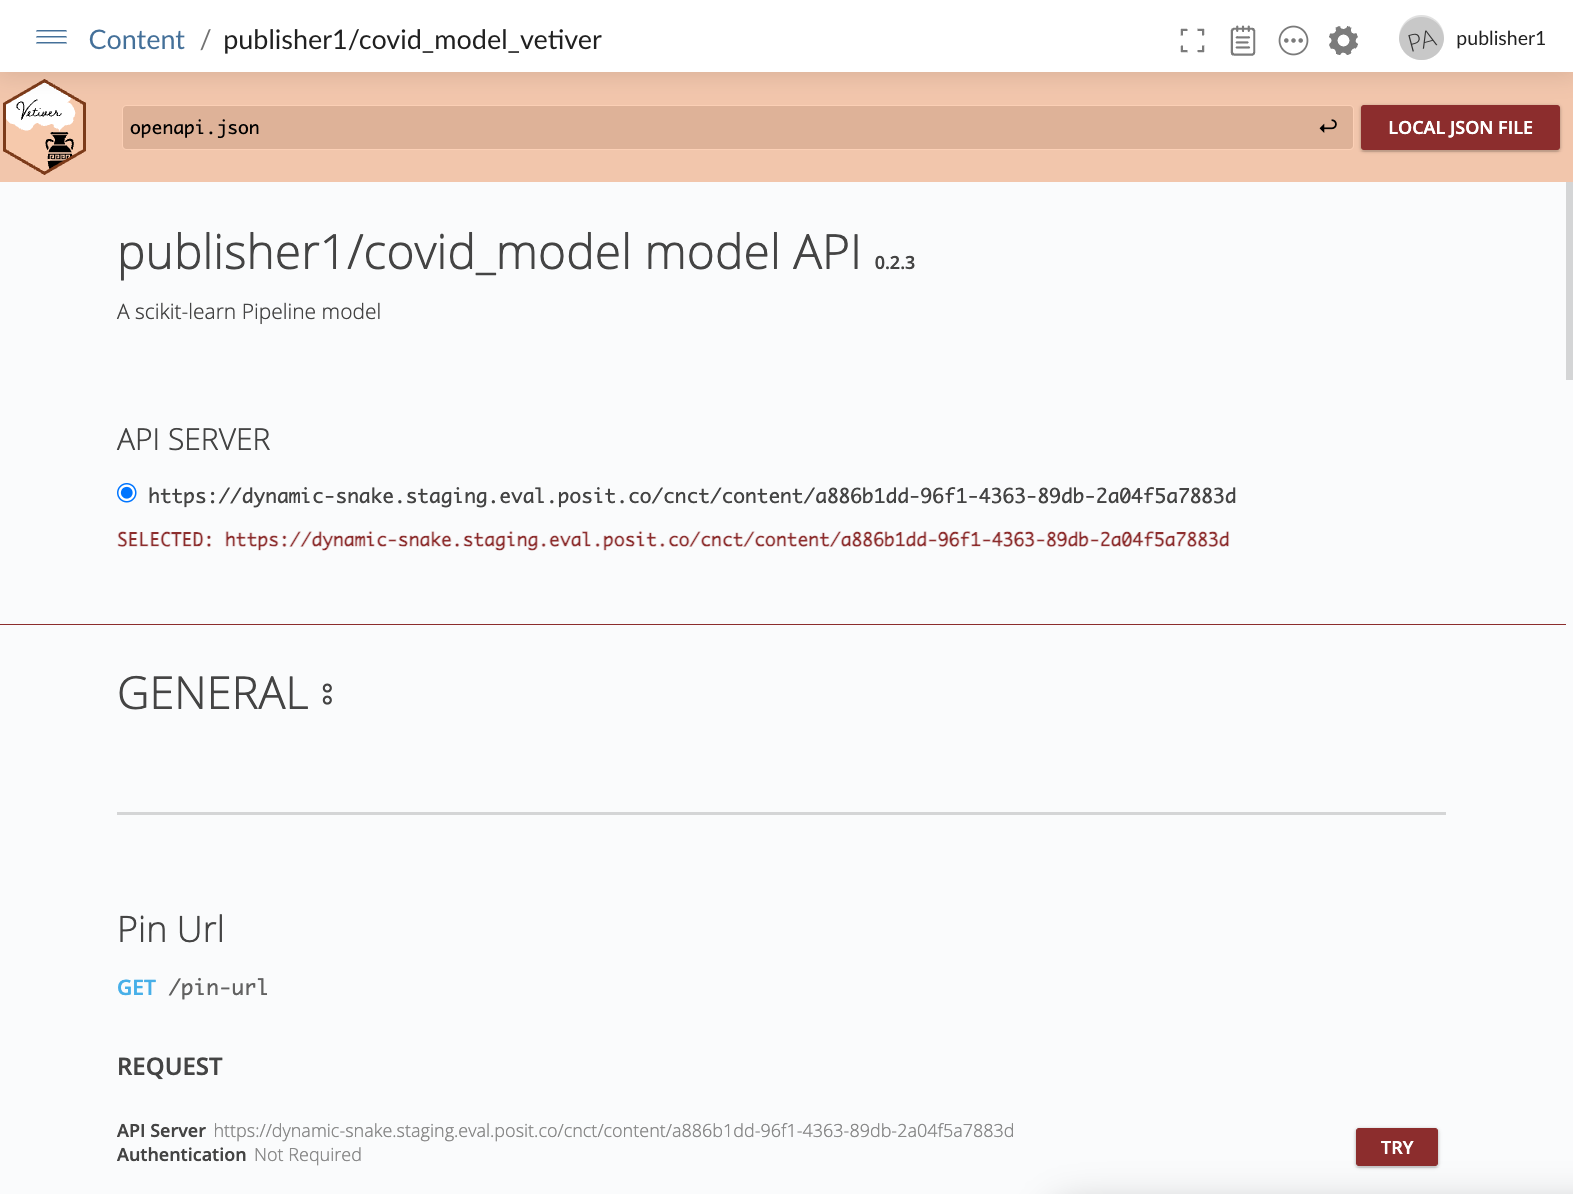
\includegraphics{images/fastapi-rapidoc.png}

}

\caption{\label{fig-fastapi-rapidoc}RapiDoc documentation for a FastAPI
hosted on Posit Connect}

\end{figure}%

This example API uses a model to predict the number of COVID cases given
a specific day of the year. You will create a similar API in the next
exercise! The prediction is generated by sending a \textbf{POST} request
to the API with specific parameters. In this case, there is only one
parameter, the day of the year (\texttt{DayOfYear}). RapiDoc allows you
to try out the API. In the image below, we asked the API to return the
prediction of the number of COVID cases on day 46 of the year. At the
bottom, you can see the response of approximately 1,033 cases:

\begin{figure}

\centering{

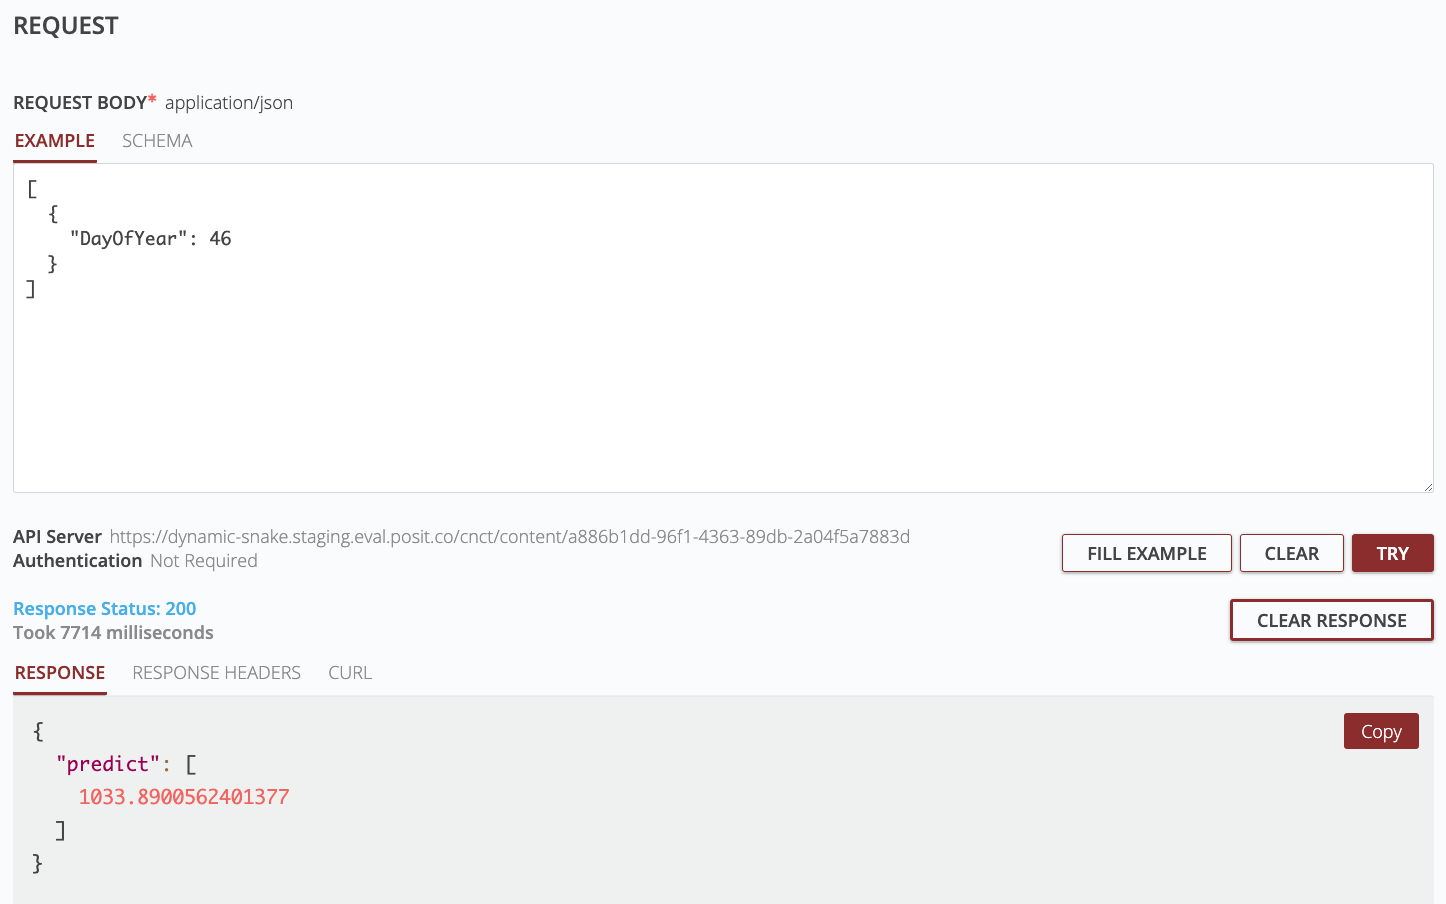
\includegraphics{images/rapidoc-response.png}

}

\caption{\label{fig-rapidoc-response}Interacting with RapiDoc}

\end{figure}%

You can also interact with APIs programmatically. In the code below,
we'll show you how to query an API using \texttt{vetiver} hosted on
Posit Connect using both R and Python. Full instructions (including
additional authentication options) can be found
\href{https://docs.posit.co/connect/user/vetiver/}{here}.

\section{Python}

\begin{Shaded}
\begin{Highlighting}[]
\ImportTok{from}\NormalTok{ vetiver.server }\ImportTok{import}\NormalTok{ predict, vetiver\_endpoint}

\CommentTok{\# Define the API endpoint}
\NormalTok{endpoint }\OperatorTok{=}\NormalTok{ vetiver\_endpoint(}
    \SpecialStringTok{f"https://connect.example.com/content/}\SpecialCharTok{\{}\NormalTok{APP\_ID}\SpecialCharTok{\}}\SpecialStringTok{/predict"}
\NormalTok{)}

\CommentTok{\# If API has restricted access, you\textquotesingle{}ll need to supply an API Key}
\NormalTok{api\_key}\OperatorTok{=}\NormalTok{os.getenv(}\StringTok{"CONNECT\_API\_KEY"}\NormalTok{)}

\CommentTok{\# Predict using new data!}
\NormalTok{h }\OperatorTok{=}\NormalTok{ \{}\StringTok{"Authorization"}\NormalTok{: }\SpecialStringTok{f"Key }\SpecialCharTok{\{}\NormalTok{api\_key}\SpecialCharTok{\}}\SpecialStringTok{"}\NormalTok{\}}
\NormalTok{response }\OperatorTok{=}\NormalTok{ predict(endpoint}\OperatorTok{=}\NormalTok{endpoint, data}\OperatorTok{=}\NormalTok{new\_data, headers}\OperatorTok{=}\NormalTok{h)}
\end{Highlighting}
\end{Shaded}

\section{R}

\begin{Shaded}
\begin{Highlighting}[]
\CommentTok{\# Define the API endpoint}
\NormalTok{endpoint }\OtherTok{\textless{}{-}} \FunctionTok{vetiver\_endpoint}\NormalTok{(}
  \StringTok{"https://connect.example.com/content/$APP\_ID/predict"}\NormalTok{)}

\CommentTok{\# If API has restricted access, you\textquotesingle{}ll need to supply an API Key}
\NormalTok{apiKey }\OtherTok{\textless{}{-}} \FunctionTok{Sys.getenv}\NormalTok{(}\StringTok{"CONNECT\_API\_KEY"}\NormalTok{)}

\CommentTok{\# Predict using new data!}
\FunctionTok{predict}\NormalTok{(}
\NormalTok{  endpoint,}
\NormalTok{  new\_data,}
\NormalTok{  httr}\SpecialCharTok{::}\FunctionTok{add\_headers}\NormalTok{(}\AttributeTok{Authorization =} \FunctionTok{paste}\NormalTok{(}\StringTok{"Key"}\NormalTok{, apiKey)))}
\end{Highlighting}
\end{Shaded}

\chapter{Exercise: Modelling}\label{sec-exercise-modelling}

\begin{figure}

\centering{

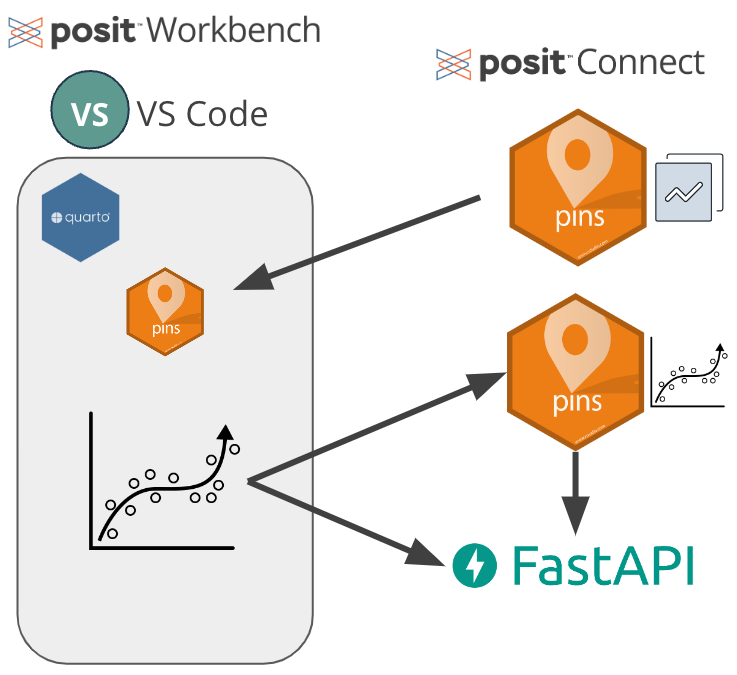
\includegraphics[width=5.15625in,height=\textheight]{images/model-workflow.png}

}

\caption{\label{fig-model-workflow}Model Workflow}

\end{figure}%

Now that we have a polished dataset pinned to Posit Connect, it's time
to \emph{understand} what the data is telling us. Furthermore, we can
use the data to train a model to help predict future events. However,
\textbf{this workshop is not a modeling workshop!} The model we will
create in this exercise is a proof-of-concept and will not be
particularly informative.

In this exercise (as shown in Figure~\ref{fig-model-workflow}), you
will:

\begin{enumerate}
\def\labelenumi{\arabic{enumi}.}
\tightlist
\item
  Read in the pinned COVID data
\item
  Use data to create a linear regression model in Posit Workbench (VS
  Code)
\item
  Pin the model to Posit Connect
\item
  Serve the pinned model as a FastAPI on Posit Connect
\end{enumerate}

\section{Step 1 - Create a Model}\label{step-1---create-a-model}

The COVID dataset contains a column (\texttt{new\_cases}) that shows how
many new cases of COVID were reported on a specific day. There is
seasonality for certain infections (e.g., influenza and RSV), and we can
use this COVID dataset to determine if the same applies to COVID. In
other words:

\begin{quote}
Can we predict new cases of COVID given a specific day of the year?
\end{quote}

To highlight the cross-language functionality of Posit Team, we will
create this model using Python! There are so many amazing packages and
modules available in Python for creating models including Tensorflow,
Keras, and SciKit-Learn. For this workshop we are going to create a
simple linear regression model using SciKit-Learn.

\subsection{Load Necessary Packages}\label{load-necessary-packages-1}

\begin{Shaded}
\begin{Highlighting}[]
\ImportTok{import}\NormalTok{ pandas }\ImportTok{as}\NormalTok{ pd}
\ImportTok{import}\NormalTok{ numpy }\ImportTok{as}\NormalTok{ np}
\ImportTok{from}\NormalTok{ sklearn.model\_selection }\ImportTok{import}\NormalTok{ train\_test\_split}
\ImportTok{from}\NormalTok{ sklearn.linear\_model }\ImportTok{import}\NormalTok{ LinearRegression}
\ImportTok{from}\NormalTok{ sklearn.pipeline }\ImportTok{import}\NormalTok{ make\_pipeline}
\ImportTok{from}\NormalTok{ sklearn.preprocessing }\ImportTok{import}\NormalTok{ PolynomialFeatures}
\ImportTok{import}\NormalTok{ matplotlib.pyplot }\ImportTok{as}\NormalTok{ plt}
\end{Highlighting}
\end{Shaded}

\subsection{Read in Pinned COVID Data}\label{read-in-pinned-covid-data}

\textbf{Reminder}: You'll need to replace \texttt{your\_name} with your
Posit Connect username in all subsequent code blocks.

\begin{Shaded}
\begin{Highlighting}[]
\ImportTok{import}\NormalTok{ pins}

\NormalTok{board }\OperatorTok{=}\NormalTok{ pins.board\_connect(allow\_pickle\_read}\OperatorTok{=}\VariableTok{True}\NormalTok{)}

\NormalTok{covid }\OperatorTok{=}\NormalTok{ board.pin\_read(}\StringTok{"your\_name/covid\_data"}\NormalTok{)}
\end{Highlighting}
\end{Shaded}

\subsection{Transform Data}\label{transform-data}

Before we can model the COVID data with SciKit-Learn, we need to
transform it to a format that is conducive to modeling. In the next
steps we will convert the date colum to a date \emph{class}, engineer a
new feature called \texttt{DayOfYear}, and select only the columns of
interest (\texttt{DayOfYear} and \texttt{new\_cases}).

\begin{Shaded}
\begin{Highlighting}[]
\CommentTok{\# Convert to date class}
\NormalTok{covid[}\StringTok{"date"}\NormalTok{] }\OperatorTok{=}\NormalTok{ pd.to\_datetime(covid[}\StringTok{"date"}\NormalTok{])}

\CommentTok{\# Feature engineering: Extracting day of the year as a feature}
\NormalTok{covid[}\StringTok{"DayOfYear"}\NormalTok{] }\OperatorTok{=}\NormalTok{ covid[}\StringTok{"date"}\NormalTok{].dt.dayofyear}

\CommentTok{\# Extract columns of interest}
\NormalTok{df }\OperatorTok{=}\NormalTok{ covid[[}\StringTok{"DayOfYear"}\NormalTok{, }\StringTok{"new\_cases"}\NormalTok{]]}
\end{Highlighting}
\end{Shaded}

\subsection{Train Linear Regression
Model}\label{train-linear-regression-model}

\begin{Shaded}
\begin{Highlighting}[]
\CommentTok{\# Create and train a linear regression model}
\NormalTok{covid\_model }\OperatorTok{=}\NormalTok{ make\_pipeline(PolynomialFeatures(}\DecValTok{4}\NormalTok{), LinearRegression()).fit(df.drop(columns}\OperatorTok{=}\StringTok{"new\_cases"}\NormalTok{), df[}\StringTok{"new\_cases"}\NormalTok{])}
\end{Highlighting}
\end{Shaded}

\section{Step 2 - Make Predictions}\label{step-2---make-predictions}

Let's use our new model to make prediction of how many new cases of
COVID there will be given a day of the year. We'll visualize these
predictions using \texttt{matplotlib}.

\begin{tcolorbox}[enhanced jigsaw, toprule=.15mm, title=\textcolor{quarto-callout-warning-color}{\faExclamationTriangle}\hspace{0.5em}{Warning}, opacitybacktitle=0.6, titlerule=0mm, arc=.35mm, bottomrule=.15mm, rightrule=.15mm, colbacktitle=quarto-callout-warning-color!10!white, coltitle=black, colframe=quarto-callout-warning-color-frame, left=2mm, opacityback=0, colback=white, breakable, bottomtitle=1mm, toptitle=1mm, leftrule=.75mm]

Your predictions/plots may look different depending on which
state/province you selected in the previous exercise.

\end{tcolorbox}

\begin{Shaded}
\begin{Highlighting}[]
\CommentTok{\# Make predictions}
\NormalTok{covid\_pred }\OperatorTok{=}\NormalTok{ covid\_model.predict(df.drop(columns}\OperatorTok{=}\StringTok{"new\_cases"}\NormalTok{))}

\CommentTok{\# Visualize the results}
\NormalTok{plt.scatter(df.drop(columns}\OperatorTok{=}\StringTok{"new\_cases"}\NormalTok{), df[}\StringTok{"new\_cases"}\NormalTok{], color}\OperatorTok{=}\StringTok{\textquotesingle{}black\textquotesingle{}}\NormalTok{, label}\OperatorTok{=}\StringTok{\textquotesingle{}Actual\textquotesingle{}}\NormalTok{)}
\NormalTok{plt.scatter(df.drop(columns}\OperatorTok{=}\StringTok{"new\_cases"}\NormalTok{), covid\_pred, color}\OperatorTok{=}\StringTok{\textquotesingle{}blue\textquotesingle{}}\NormalTok{, s}\OperatorTok{=}\DecValTok{2}\NormalTok{, label}\OperatorTok{=}\StringTok{\textquotesingle{}Predicted\textquotesingle{}}\NormalTok{)}
\NormalTok{plt.xlabel(}\StringTok{\textquotesingle{}Day of Year\textquotesingle{}}\NormalTok{)}
\NormalTok{plt.ylabel(}\StringTok{\textquotesingle{}Number of Cases\textquotesingle{}}\NormalTok{)}
\NormalTok{plt.legend()}
\NormalTok{plt.show()}
\end{Highlighting}
\end{Shaded}

\begin{figure}

\centering{

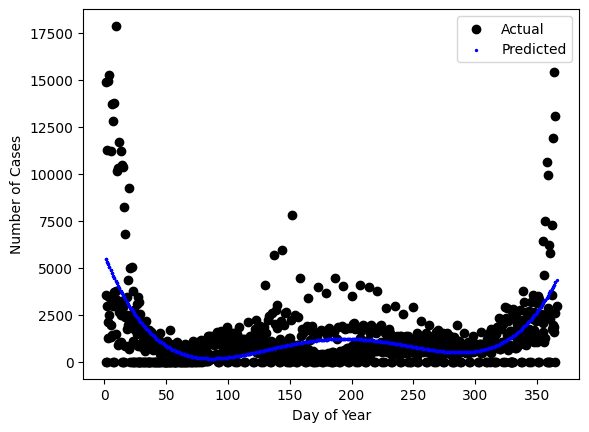
\includegraphics{images/covid-predictions.png}

}

\caption{\label{fig-covid-predictions}New cases of COVID for Maryland}

\end{figure}%

\section{Step 3 - Save and Serve
Model}\label{step-3---save-and-serve-model}

In the next steps, we'll convert our linear regression model to a
\emph{vetiver model} and subsequently save it as a pin to Posit Connect.
We'll then use the pinned model to create a FastAPI that will serve our
model so we can interact with it.

\subsection{Create a Vetiver Model}\label{create-a-vetiver-model}

\begin{Shaded}
\begin{Highlighting}[]
\ImportTok{from}\NormalTok{ vetiver }\ImportTok{import}\NormalTok{ VetiverModel}

\CommentTok{\# Create Vetiver model}
\NormalTok{v }\OperatorTok{=}\NormalTok{ VetiverModel(covid\_model, model\_name }\OperatorTok{=} \StringTok{"publisher1/covid\_model"}\NormalTok{, prototype\_data}\OperatorTok{=}\NormalTok{df.drop(columns}\OperatorTok{=}\StringTok{"new\_cases"}\NormalTok{))}
\end{Highlighting}
\end{Shaded}

\subsection{Save Model as a Pin to Posit
Connect}\label{save-model-as-a-pin-to-posit-connect}

\begin{Shaded}
\begin{Highlighting}[]
\ImportTok{from}\NormalTok{ vertiver }\ImportTok{import}\NormalTok{ vetiver\_pin\_write}

\CommentTok{\# Save model as pin to Posit Connect. The "board"" was defined above}
\NormalTok{vetiver\_pin\_write(board, v)}
\end{Highlighting}
\end{Shaded}

\subsection{Serve Model as a FastAPI on Posit
Connect}\label{serve-model-as-a-fastapi-on-posit-connect}

In the below code, we will use the pinned model to serve a FastAPI. For
our workshop environment, the \texttt{CONNECT\_SERVER} and
\texttt{CONNECT\_API\_KEY} variables are already present in your
environment, and you'll use the \texttt{os} package to retrieve them.

\begin{Shaded}
\begin{Highlighting}[]
\ImportTok{from}\NormalTok{ vetiver }\ImportTok{import}\NormalTok{ VetiverAPI, deploy\_rsconnect}
\ImportTok{from}\NormalTok{ rsconnect.api }\ImportTok{import}\NormalTok{ RSConnectServer}

\CommentTok{\# Define Connect Server}
\NormalTok{connect\_server }\OperatorTok{=}\NormalTok{ RSConnectServer(}
\NormalTok{    url}\OperatorTok{=}\NormalTok{os.getenv(}\StringTok{"CONNECT\_SERVER"}\NormalTok{)}
\NormalTok{    api\_key}\OperatorTok{=}\NormalTok{os.getenv(}\StringTok{"CONNECT\_API\_KEY"}\NormalTok{))}
    
\CommentTok{\# Deploy FastAPI    }
\NormalTok{deploy\_rsconnect(board }\OperatorTok{=}\NormalTok{ board, }
\NormalTok{                 pin\_name }\OperatorTok{=} \StringTok{"publisher1/covid\_model"}\NormalTok{, }
\NormalTok{                 connect\_serve}\OperatorTok{==}\NormalTok{connect\_server)}
\end{Highlighting}
\end{Shaded}

\section{Step 4 - Interact with
FastAPI}\label{step-4---interact-with-fastapi}

With the FastAPI now deployed to Posit Connect, we can programmatically
query the API which will return the predicted number of new COVID cases
given a specific day of the year. Before we query the API, there are a
few variable we should set including the endpoint as well as the query
parameters:

\begin{Shaded}
\begin{Highlighting}[]
\ImportTok{import}\NormalTok{ os}
\ImportTok{import}\NormalTok{ pandas }\ImportTok{as}\NormalTok{ pd}
\ImportTok{from}\NormalTok{ vetiver.server }\ImportTok{import}\NormalTok{ predict, vetiver\_endpoint}

\CommentTok{\# Set vetiver endpoing (URL can be found on Posit Connect)}
\CommentTok{\#  Might need to add "predict" to the end of the URL}
\NormalTok{endpoint }\OperatorTok{=}\NormalTok{ vetiver\_endpoint(}\StringTok{"https://connectexample.posit.co/cnct/content/}\SpecialCharTok{\{APP\_ID\}}\StringTok{/predict"}\NormalTok{)}

\CommentTok{\# Define API key (if not done already)}
\NormalTok{api\_key }\OperatorTok{=}\NormalTok{ os.getenv(}\StringTok{"CONNECT\_API\_KEY"}\NormalTok{)}

\CommentTok{\# Define query parameters. Example: 44th day of the year}
\NormalTok{params }\OperatorTok{=}\NormalTok{ pd.DataFrame(\{}\StringTok{\textquotesingle{}DayOfYear\textquotesingle{}}\NormalTok{: [}\DecValTok{44}\NormalTok{]\})}

\CommentTok{\# Query API!}
\NormalTok{h }\OperatorTok{=}\NormalTok{ \{}\StringTok{"Authorization"}\NormalTok{: }\SpecialStringTok{f"Key }\SpecialCharTok{\{}\NormalTok{api\_key}\SpecialCharTok{\}}\SpecialStringTok{"}\NormalTok{\}}
\NormalTok{predict(endpoint}\OperatorTok{=}\NormalTok{endpoint, data}\OperatorTok{=}\NormalTok{params, headers}\OperatorTok{=}\NormalTok{h)}
\end{Highlighting}
\end{Shaded}

\part{Communicate}

\chapter{Shiny}\label{shiny}

\begin{center}

\includegraphics{images/shiny.png}
\end{center}

You might invest days, weeks, or even months developing an impressive
data science workflow and your confident that the results of your
workflow are brimming with \emph{value} - value to you, your colleagues,
your clients, or decision makers at your company.

Failure to \textbf{communicate} the results of your workflow to the
pertinent parties leads to a loss of value. As such, it's worth
investing in strategies that can make your workflow results ``shine
bright'' for all to see and consume. Enter
\href{https://shiny.posit.co/}{\texttt{shiny}}!

Shiny is an open-source R and Python package and is used to build
\emph{interactive web applications}. The best part? You don't have to be
a web developer to create a shiny app! You just need to know a bit of R
and/or Python. Shiny is 100\% code-based, which sets it apart from other
popular business intelligence (BI) tools.

\section{What's in a Shiny App?}\label{whats-in-a-shiny-app}

Most shiny applications have 4 components:

\begin{itemize}
\item
  \textbf{Header:} The header is usually at the very top of the shiny
  application. This is a useful space for things that need to be
  executed as soon as someone opens your shiny application such as
  reading in any data or packages.
\item
  \textbf{User Interface (UI):} The UI is where design the visual layout
  of your application. Specifically where to put your inputs and
  outputs.
\item
  \textbf{Server Function:} The server function tells shiny \emph{how}
  to build the various outputs.
\item
  \textbf{Run app:} This is where you combine the UI and Server function
  into a single shiny application.
\end{itemize}

Below is the code for a simple shiny application, written in both R and
Python:

\section{Python}

\begin{Shaded}
\begin{Highlighting}[]
\CommentTok{\# Header}
\ImportTok{from}\NormalTok{ shiny }\ImportTok{import} \OperatorTok{*}

\CommentTok{\# UI}
\NormalTok{app\_ui }\OperatorTok{=}\NormalTok{ ui.page\_fluid(}
\NormalTok{    ui.input\_slider(}\StringTok{"n"}\NormalTok{, }\StringTok{"N"}\NormalTok{, }\DecValTok{1}\NormalTok{, }\DecValTok{100}\NormalTok{, }\DecValTok{40}\NormalTok{),}
\NormalTok{    ui.output\_text\_verbatim(}\StringTok{"txt"}\NormalTok{),}
\NormalTok{)}

\CommentTok{\# Server Function}
\KeywordTok{def}\NormalTok{ server(}\BuiltInTok{input}\NormalTok{, output, session):}
    \AttributeTok{@output}
    \AttributeTok{@render.text}
    \KeywordTok{def}\NormalTok{ txt():}
        \ControlFlowTok{return} \SpecialStringTok{f"The value of n*2 is }\SpecialCharTok{\{}\BuiltInTok{input}\SpecialCharTok{.}\NormalTok{n() }\OperatorTok{*} \DecValTok{2}\SpecialCharTok{\}}\SpecialStringTok{"}

\CommentTok{\# Run App}
\NormalTok{app }\OperatorTok{=}\NormalTok{ App(app\_ui, server)}
\end{Highlighting}
\end{Shaded}

\section{R}

\begin{Shaded}
\begin{Highlighting}[]
\CommentTok{\# Header}
\FunctionTok{library}\NormalTok{(shiny)}

\CommentTok{\# UI}
\NormalTok{ui }\OtherTok{\textless{}{-}} \FunctionTok{fluidPage}\NormalTok{(}
  \FunctionTok{sliderInput}\NormalTok{(}\StringTok{"n"}\NormalTok{, }\StringTok{"N"}\NormalTok{, }\DecValTok{1}\NormalTok{, }\DecValTok{100}\NormalTok{, }\DecValTok{40}\NormalTok{),}
  \FunctionTok{textOutput}\NormalTok{(}\StringTok{"txt"}\NormalTok{)}
  
\NormalTok{)}

\CommentTok{\# Server Function}
\NormalTok{server }\OtherTok{\textless{}{-}} \ControlFlowTok{function}\NormalTok{(input, output) \{}
\NormalTok{  output}\SpecialCharTok{$}\NormalTok{txt }\OtherTok{\textless{}{-}} \FunctionTok{renderText}\NormalTok{(\{}
    \FunctionTok{paste0}\NormalTok{(}\StringTok{"The value of n*2 is: "}\NormalTok{, input}\SpecialCharTok{$}\NormalTok{n }\SpecialCharTok{*} \DecValTok{2}\NormalTok{)}
\NormalTok{  \})}
\NormalTok{\}}

\CommentTok{\# Run App}
\FunctionTok{shinyApp}\NormalTok{(}\AttributeTok{ui =}\NormalTok{ ui, }\AttributeTok{server =}\NormalTok{ server)}
\end{Highlighting}
\end{Shaded}

\section{Incorporating Shiny into your
Workflow}\label{incorporating-shiny-into-your-workflow}

\begin{figure}

\centering{

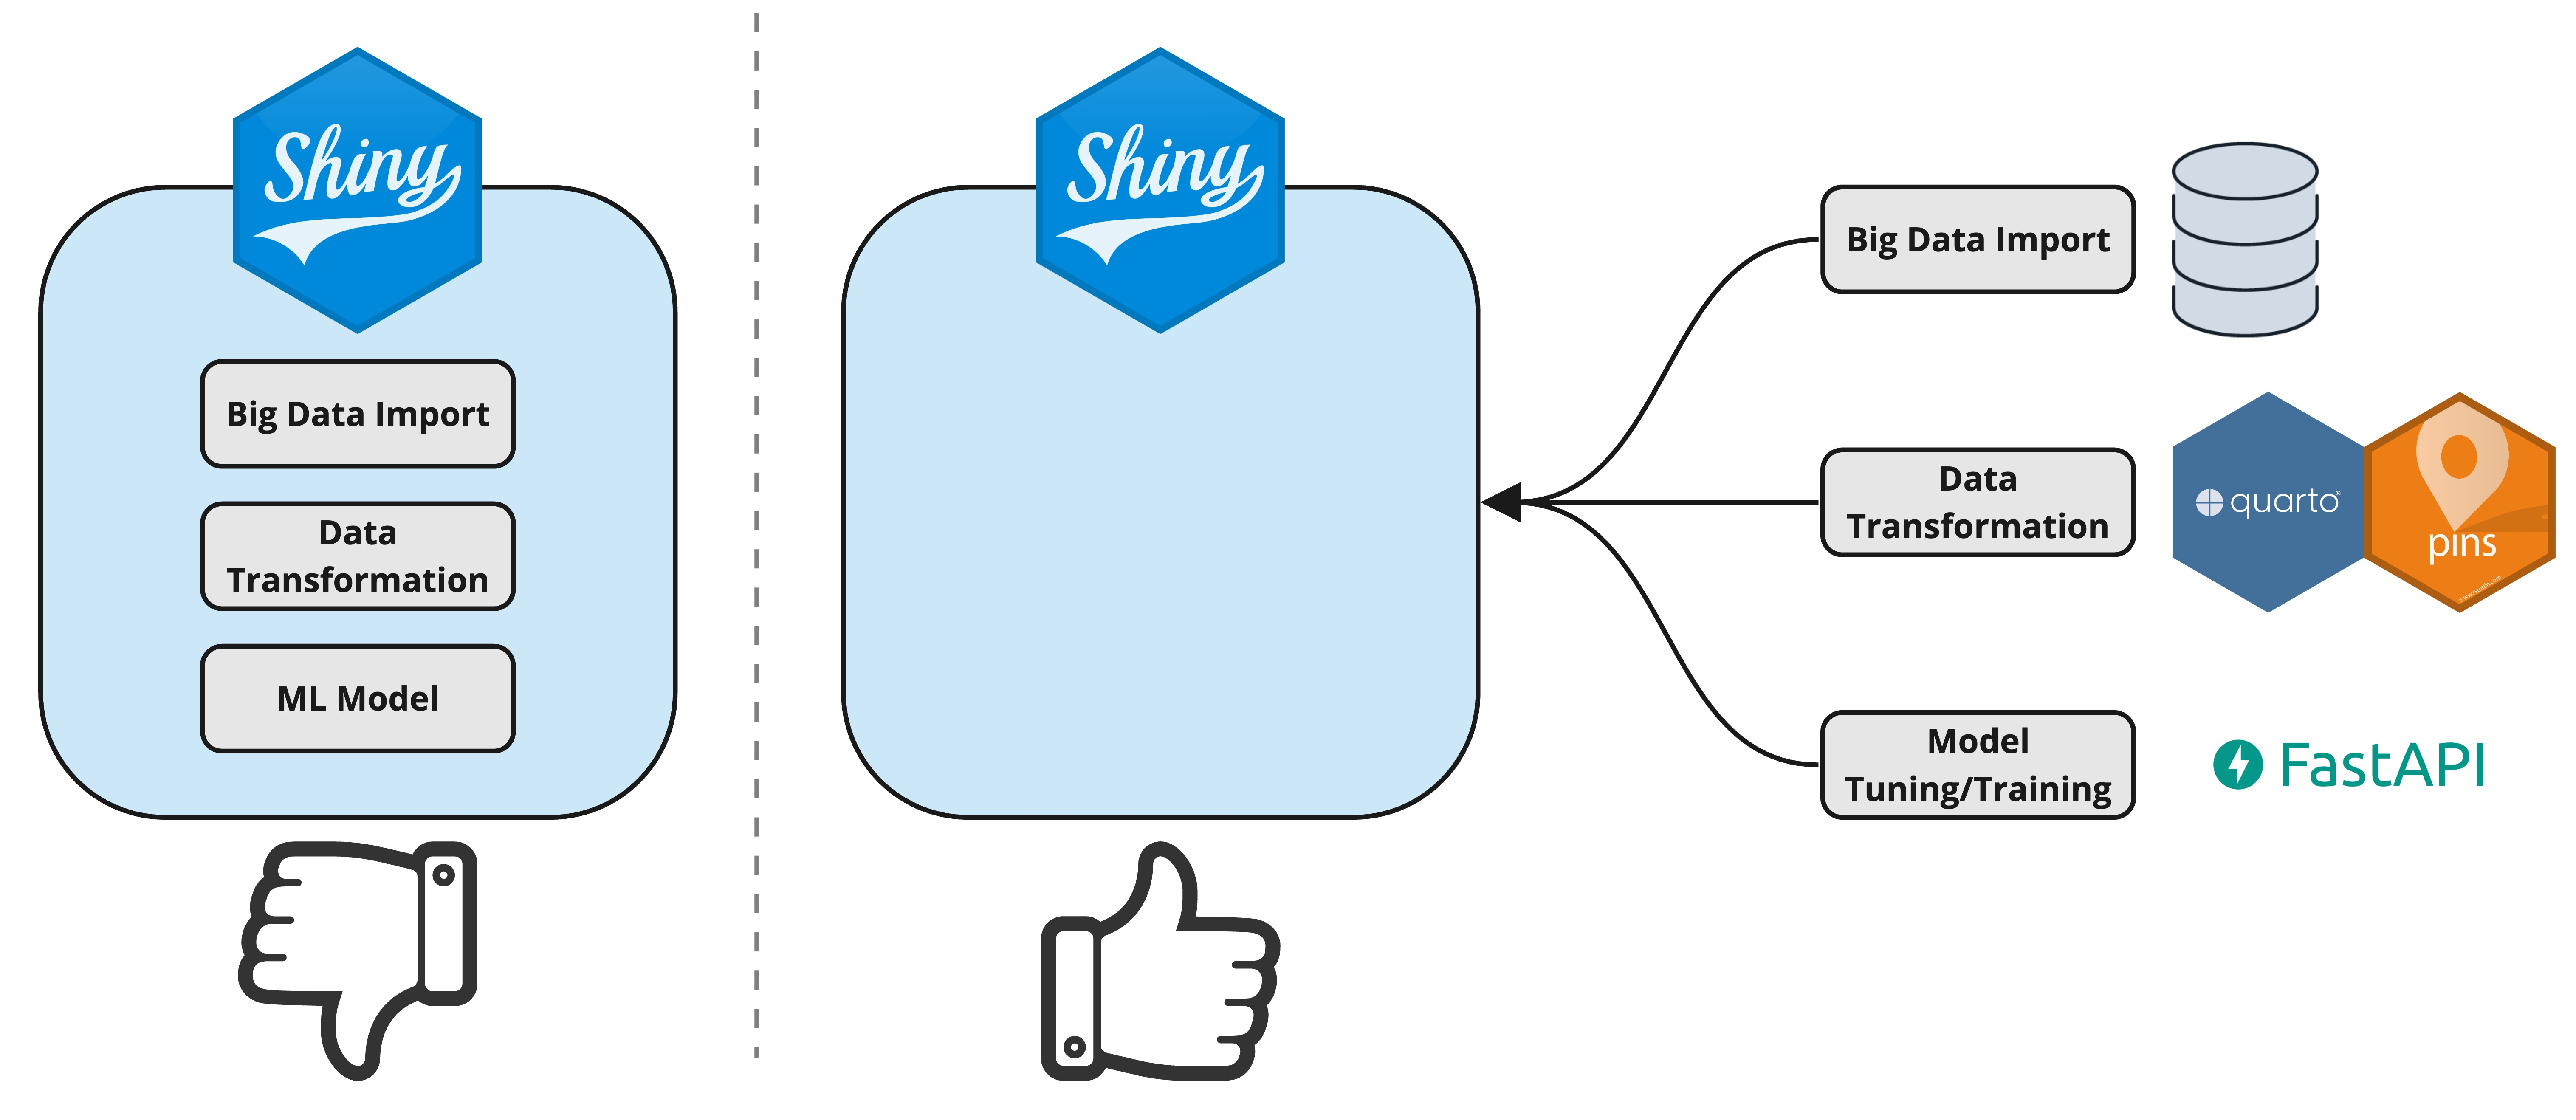
\includegraphics{images/shiny-prod.jpg}

}

\caption{\label{fig-shiny-prod}Shiny application best practices}

\end{figure}%

It can be tempting to incorporate your \emph{entire} data science
workflow into your shiny application. This often leads to bloated
applications that are frustratingly slow (see left side of
Figure~\ref{fig-shiny-prod}). Instead, it's recommended to decouple the
``computationally heavy'' parts of your workflow from your shiny
application where possible (see right side of
Figure~\ref{fig-shiny-prod}). Consider the two examples below (both of
which we've discussed in previous chapters):

\begin{itemize}
\item
  If your shiny application relies on large datasets, make sure to only
  read in the data required for the application. Also consider
  pre-processing your data before reading it into the shiny application.
\item
  If your shiny application leverages a machine learning model, consider
  training/tuning your model outside of shiny and serving it as an API.
\end{itemize}

By keeping the steps of your workflow independent from each other, you
can dramatically improve your shiny application's performance and
simplify the underlying code. These are two big steps for making your
shiny applications more \textbf{production grade!}

\chapter{Exercise: Shiny for Python}\label{sec-exercise-shiny-py}

\begin{figure}

\centering{


\includegraphics[width=4.625in,height=\textheight]{images/shiny-fastapi.png}

}

\caption{\label{fig-shiny-fastapi}Shiny + FastAPI workflow}

\end{figure}%

In this exercise, you will get practice creating a Shiny or Python
application in Posit Workbench (VS Code) that makes predictions of new
cases of COVID given a specific day of the year. This shiny application
will be fairly ``lightweight'' in that it's primary role is to query the
FastAPI on Posit Connect that serving our COVID model we created earlier
in Chapter~\ref{sec-exercise-modelling}. The user interface will only
contain two things: a date selection box, and a text box with the
predicted number of COVID cases:

\begin{figure}

\centering{

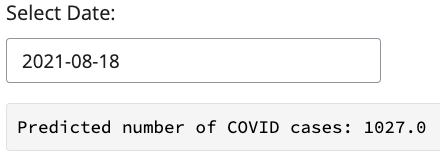
\includegraphics{images/shiny-ui-py.png}

}

\caption{\label{fig-shiny-ui-py}COVID Prediction App - Shiny for Python}

\end{figure}%

\section{Step 1 - Set the Stage}\label{step-1---set-the-stage}

Before we define our Shiny app user interface and server function, we
first need to import the necessary packages and define some variables.

\subsection{Import Necessary Packages}\label{import-necessary-packages}

\begin{Shaded}
\begin{Highlighting}[]
\ImportTok{from}\NormalTok{ shiny }\ImportTok{import}\NormalTok{ App, render, ui}
\ImportTok{import}\NormalTok{ os}
\ImportTok{import}\NormalTok{ vetiver}
\ImportTok{import}\NormalTok{ pandas }\ImportTok{as}\NormalTok{ pd}
\end{Highlighting}
\end{Shaded}

\subsection{Set Variables}\label{set-variables}

The primary variable we need to set is the vetiver endpoint. You'll need
to supply the API URL which can be found on Posit Connect. The other
variable is the Posit Connect API key, which is only needed if your API
requires authenticated access.

\begin{Shaded}
\begin{Highlighting}[]
\CommentTok{\# Define endpoint for API and key}
\NormalTok{endpoint }\OperatorTok{=}\NormalTok{ vetiver.vetiver\_endpoint(}\StringTok{"https://connectexample.posit.co/cnct/content/}\SpecialCharTok{\{APP\_ID\}}\StringTok{/predict"}\NormalTok{)}

\NormalTok{api\_key }\OperatorTok{=}\NormalTok{ os.getenv(}\StringTok{"CONNECT\_API\_KEY"}\NormalTok{) }
\end{Highlighting}
\end{Shaded}

\section{Step 2 - Create User
Interface}\label{step-2---create-user-interface}

As shown in Figure~\ref{fig-shiny-ui-py}, our application only has an
\emph{input date}, and \emph{output text}.

\begin{Shaded}
\begin{Highlighting}[]
\CommentTok{\# User Interface}
\NormalTok{app\_ui }\OperatorTok{=}\NormalTok{ ui.page\_fluid(}
\NormalTok{    ui.input\_date(}\StringTok{"day"}\NormalTok{, }\StringTok{"Select Date:"}\NormalTok{, value}\OperatorTok{=}\StringTok{"2021{-}01{-}01"}\NormalTok{),}
\NormalTok{    ui.output\_text\_verbatim(}\StringTok{"txt"}\NormalTok{)}
\NormalTok{)}
\end{Highlighting}
\end{Shaded}

\section{Step 3 - Create Server
Function}\label{step-3---create-server-function}

The goal of the server function is to query the FastAPI and use the API
response to create the text output. After the server function, be sure
to call the \texttt{App} function to bring together our UI and server
function into a single app object!

\begin{Shaded}
\begin{Highlighting}[]
\CommentTok{\# Server Function}
\KeywordTok{def}\NormalTok{ server(}\BuiltInTok{input}\NormalTok{, output, session):}
    \AttributeTok{@render.text}
    \KeywordTok{def}\NormalTok{ txt():}
       
        \CommentTok{\# Parameters to be included in the query string}
        \CommentTok{\#  Convert date to number of year}
\NormalTok{        params }\OperatorTok{=}\NormalTok{ pd.DataFrame(\{}
            \StringTok{\textquotesingle{}DayOfYear\textquotesingle{}}\NormalTok{: [}\BuiltInTok{input}\NormalTok{.day().strftime(}\StringTok{"\%j"}\NormalTok{)]}
\NormalTok{        \})}

        \CommentTok{\# If needed, add authorization}
\NormalTok{        h }\OperatorTok{=}\NormalTok{ \{}\StringTok{"Authorization"}\NormalTok{: }\SpecialStringTok{f"Key }\SpecialCharTok{\{}\NormalTok{api\_key}\SpecialCharTok{\}}\SpecialStringTok{"}\NormalTok{\}}

        \CommentTok{\# Make a prediction}
\NormalTok{        response }\OperatorTok{=}\NormalTok{ vetiver.predict(endpoint}\OperatorTok{=}\NormalTok{endpoint, data}\OperatorTok{=}\NormalTok{params, headers}\OperatorTok{=}\NormalTok{h).at[}\DecValTok{0}\NormalTok{, }\StringTok{"predict"}\NormalTok{].}\BuiltInTok{round}\NormalTok{()}

        \CommentTok{\# Return message}
        \ControlFlowTok{return} \SpecialStringTok{f"Predicted number of COVID cases: }\SpecialCharTok{\{}\NormalTok{response}\SpecialCharTok{\}}\SpecialStringTok{"}
      
\CommentTok{\# Create Shiny App}
\NormalTok{app }\OperatorTok{=}\NormalTok{ App(app\_ui, server)}
\end{Highlighting}
\end{Shaded}

\section{Step 4 - Run the Application on Posit
Workbench}\label{step-4---run-the-application-on-posit-workbench}

Access the terminal within VS Code (click the three line icon in the top
left corner followed by \texttt{Terminal} --\textgreater{}
\texttt{New\ Terminal}). The workshop environment is already configured
with the \texttt{shiny} CLI tool which we can use to run the shiny
application.

To run the shiny application, make sure you've saved your application as
\texttt{app.py} and you know where it's located in your file system,
then type the following command into the terminal:

\begin{Shaded}
\begin{Highlighting}[]
\ExtensionTok{shiny}\NormalTok{ run /path/to/app.py}
\end{Highlighting}
\end{Shaded}

You'll see a link appear in the terminal that you can click, or you can
use the Posit Workbench VS Code extension (red arrow in
Figure~\ref{fig-vscode-pwb-extension}) to view actively running
``proxied servers.'' In the below example, you can see two servers
running. The bottom server is actively running our shiny app!

\begin{figure}

\centering{

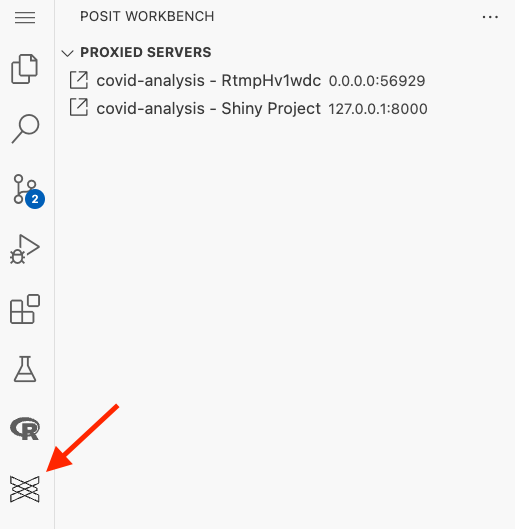
\includegraphics[width=4.14583in,height=\textheight]{images/vscode-pwb-extension.png}

}

\caption{\label{fig-vscode-pwb-extension}Posit Workbench VS Code
Extension}

\end{figure}%

\section{Step 5 - Publish Shiny Application to Posit
Connect}\label{step-5---publish-shiny-application-to-posit-connect}

In the last step, we'll show how to use the \texttt{rsconnect-python}
CLI tool to publish our shiny for python application to Posit Connect.

The only prerequisite needed, is to define the instance of Posit Connect
you would like to publish to. In the workshop environment, this has
already been configured, and you can run \texttt{rsconnect\ list} in the
terminal to view the details. See Posit's documentation for
\href{https://docs.posit.co/rsconnect-python/\#remembering-server-information}{how
to add a new Posit Connect} instance if needed.

To publish the shiny application, run the following command in the
terminal:

\begin{Shaded}
\begin{Highlighting}[]
\ExtensionTok{rsconnect}\NormalTok{ deploy shiny path/to/app.py/}
\end{Highlighting}
\end{Shaded}

The only argument you need to supply is the directory that contains the
shiny for python application (called \texttt{app.py}). Once the
deployment process is complete, you can click the links at the bottom of
the terminal (see example terminal output below) to view the application
now hosted on Posit Connect!

\begin{Shaded}
\begin{Highlighting}[]
\ExtensionTok{Deployment}\NormalTok{ completed successfully.}
         \ExtensionTok{Dashboard}\NormalTok{ content URL: https://connectexample.posit.co/cnct/connect/\#/\{APP\_ID\}}
         \ExtensionTok{Direct}\NormalTok{ content URL: https://connectexample.posit.co/cnct/content/\{APP\_ID\}/}
\end{Highlighting}
\end{Shaded}

\chapter{Exercise: Shiny for R}\label{exercise-shiny-for-r}

\begin{figure}

\centering{

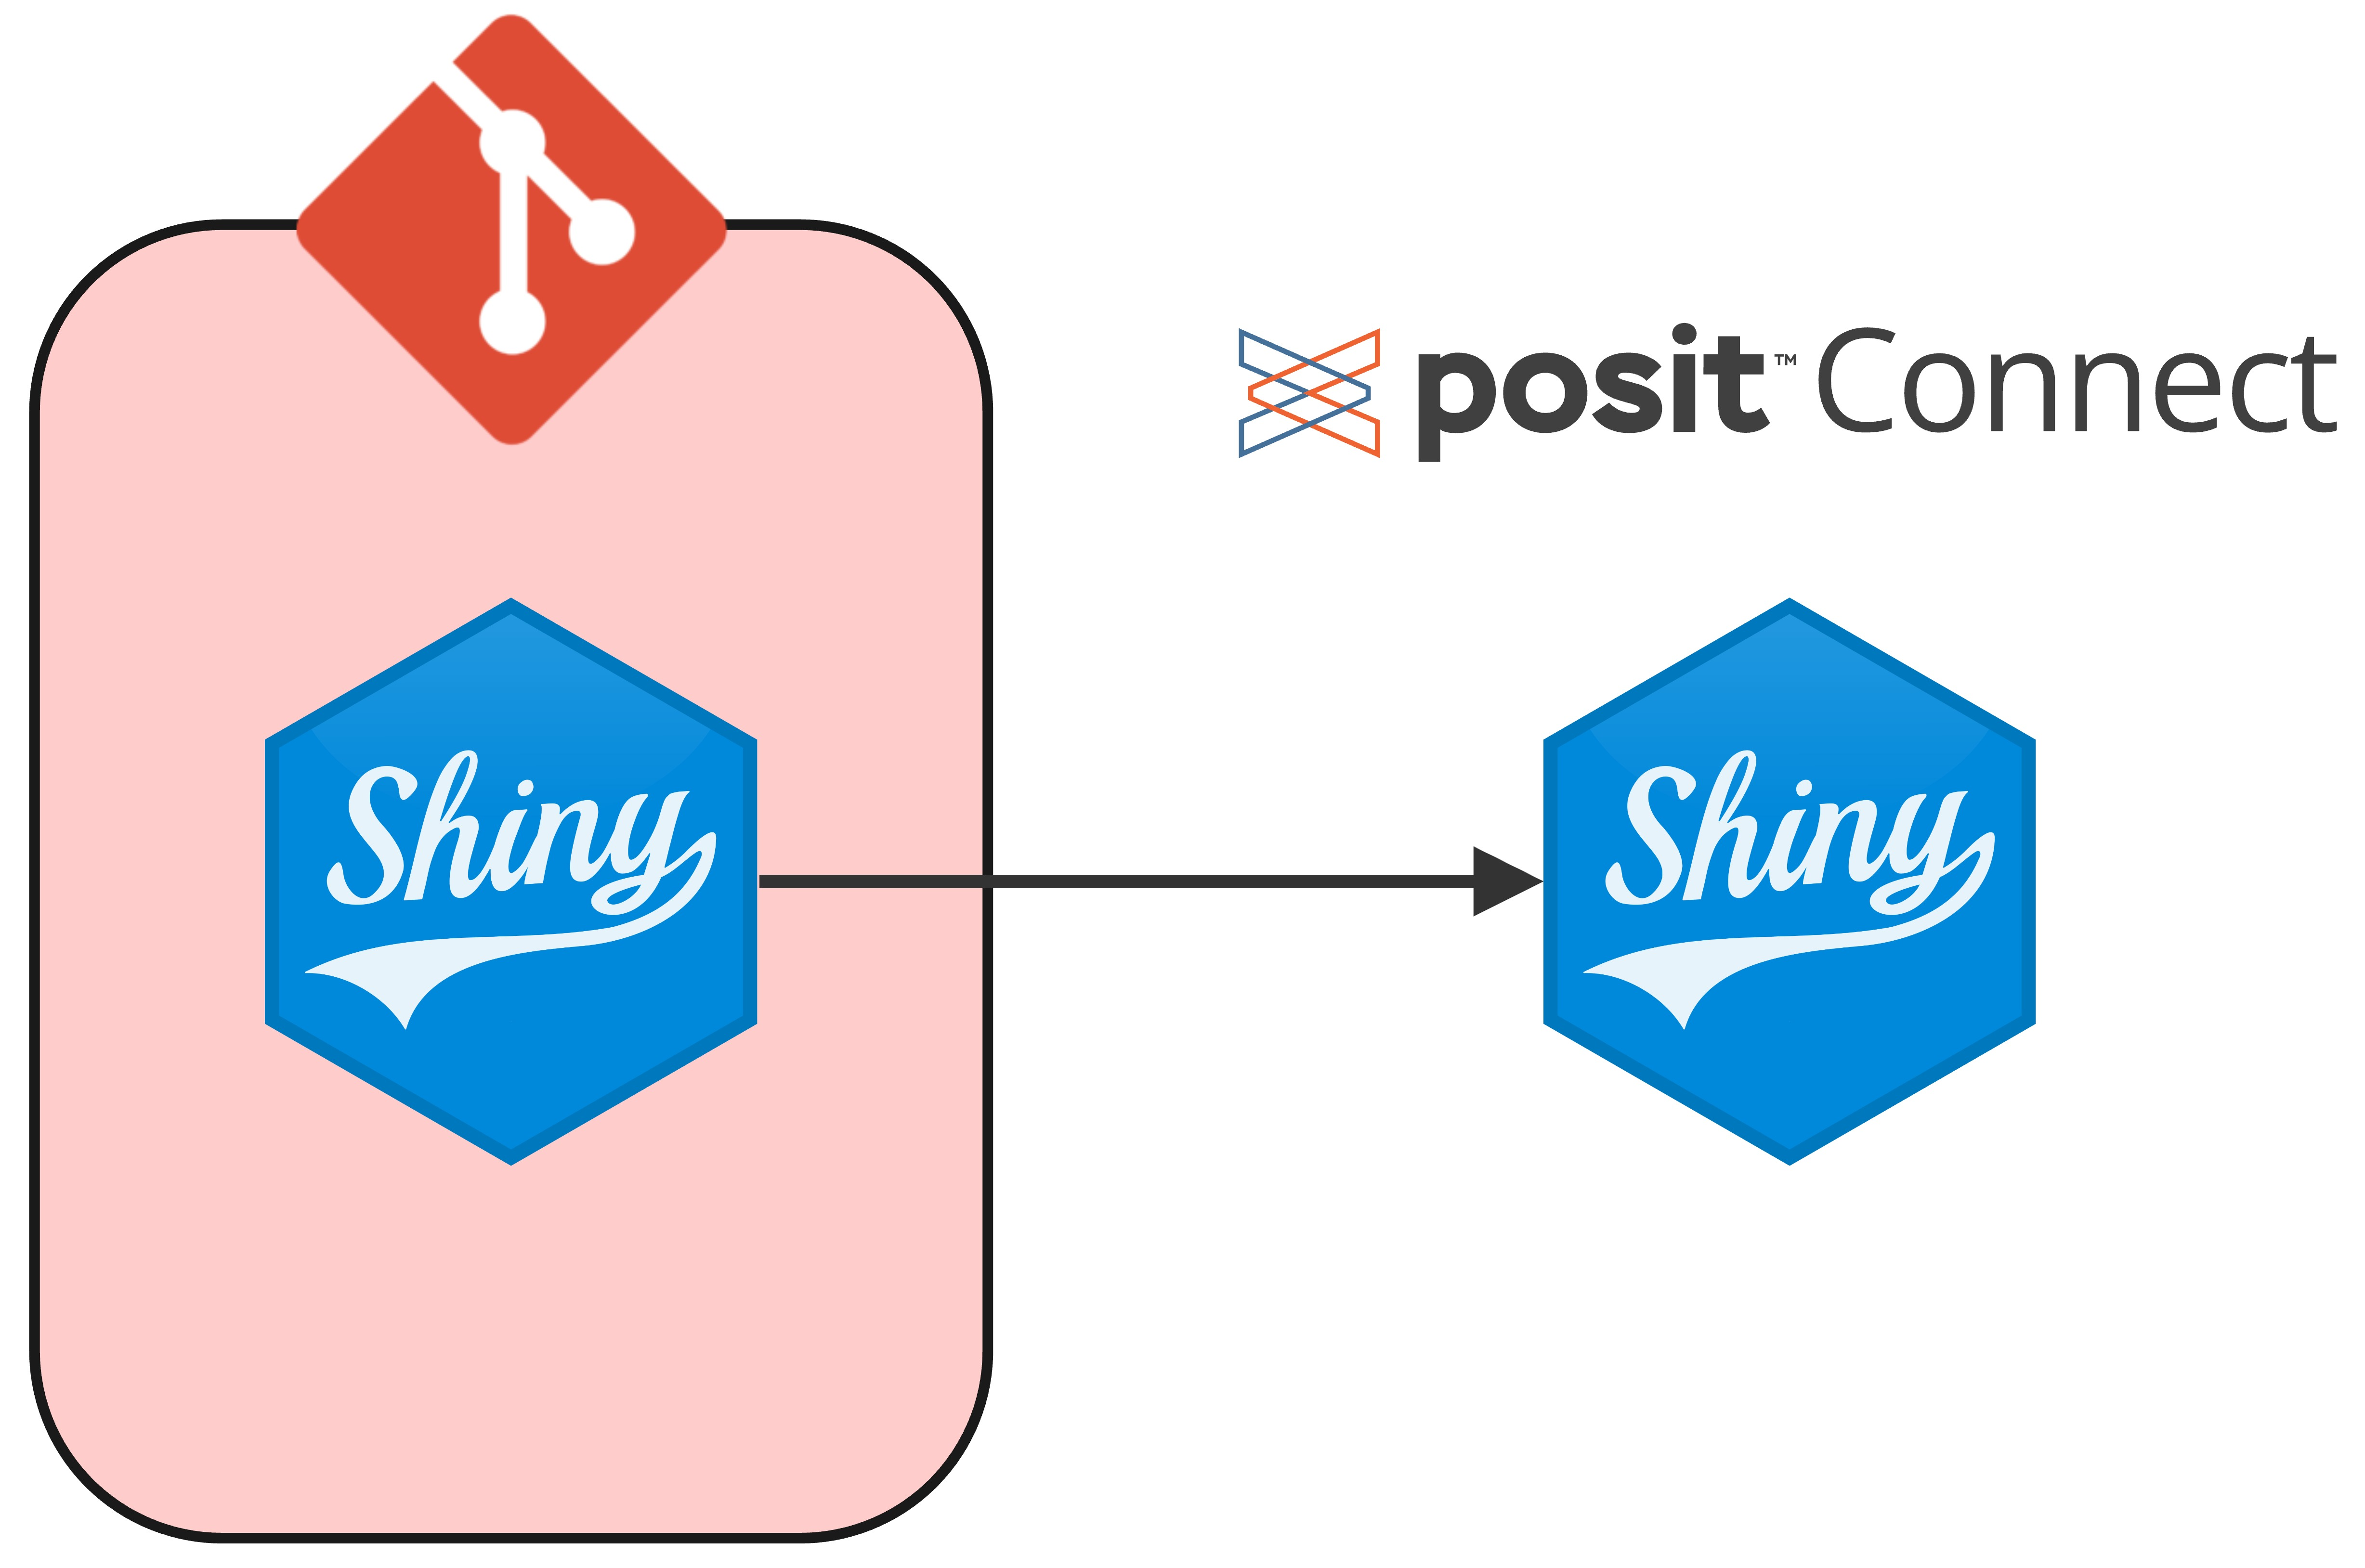
\includegraphics[width=5.27083in,height=\textheight]{images/git-backed-workflow.jpg}

}

\caption{\label{fig-git-backed-workflow}Git Backed Deployment Workflow}

\end{figure}%

In the previous exercise (Chapter~\ref{sec-exercise-shiny-py}), we
created a shiny application and \textbf{manually} deployed it to Posit
Connect. What happens if you make a change to your application? Well
you'll have to manually deploy again\ldots and again\ldots and again.

Automating manual processes can save your team time and headaches. In
this exercise, you will get practice automating the deployment process
by using git-backed deployment!

\section{Introduction to Git-Backed
Deployment}\label{introduction-to-git-backed-deployment}

Every data science workflow should use version control! The most popular
version control system is \emph{git}, which allows you to track the
evolution of your workflow's source code. You can host the tracked files
in what's known as a \emph{repository.}

If the content your working on (or maybe collaboratively working on)
lives withing in git repository, then you can publish it directly to
Posit Connect! The only requirement is you'll need to supply a companion
\texttt{manifest.json} file for your content. This file contains
information about the development environment so that Posit Connect
knows which packages, package version, and R/Python versions are needed
to run the content on Posit Connect. To create a manifest file for your
R/Python content, see the documentation
\href{https://docs.posit.co/connect/user/git-backed/}{here} and example
code snippets below:

\section{Python}

\begin{Shaded}
\begin{Highlighting}[]
\NormalTok{rsconnect write}\OperatorTok{{-}}\NormalTok{manifest}
\end{Highlighting}
\end{Shaded}

\section{R}

\begin{Shaded}
\begin{Highlighting}[]
\FunctionTok{library}\NormalTok{(rsconnect)}

\FunctionTok{writeManifest}\NormalTok{()}
\end{Highlighting}
\end{Shaded}

Once a piece of content is deployed to Posit Connect via git-backed
deployment, anytime there is an update to the content within the git
repository, Posit Connect will detect that change and
\textbf{automatically redeploy the content!}

For this exercise, we've created a
\href{https://github.com/ryjohnson09/covid-analysis/tree/main}{GitHub
repository} that contains a Shiny application (built using R) which
we'll deploy to Posit Connect.

\section{Step 1 - Initiate Git-Backed Deployment on Posit
Connect}\label{step-1---initiate-git-backed-deployment-on-posit-connect}

Within the GitHub repository is a directory called \texttt{shiny-app-r}.
Within that directory will be the two files required for git-backed
deployment: the application itself (\texttt{app.py}) and the required
\texttt{manifest.json} file.

Within Posit Connect, navigate to the \textbf{Content} page and click
the \textbf{Publish} button at the top. In the dropdown menu, select
\textbf{Import from Git}.

\begin{figure}

\centering{

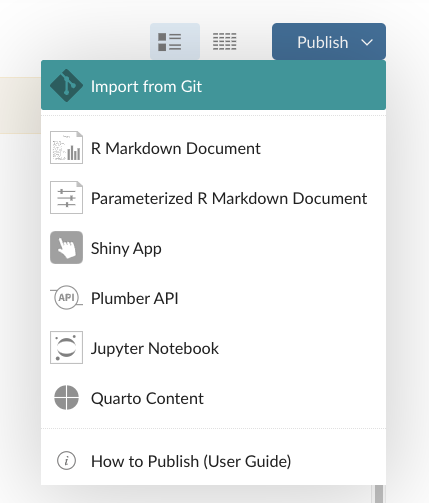
\includegraphics[width=3.34375in,height=\textheight]{images/import-from-git.png}

}

\caption{\label{fig-publish-dropdown}Publish Drop Down Options}

\end{figure}%

\section{Step 2 - Add Repository
Details}\label{step-2---add-repository-details}

In the next popup window, you'll need to supply the URL for the git
repository.

\begin{figure}

\centering{

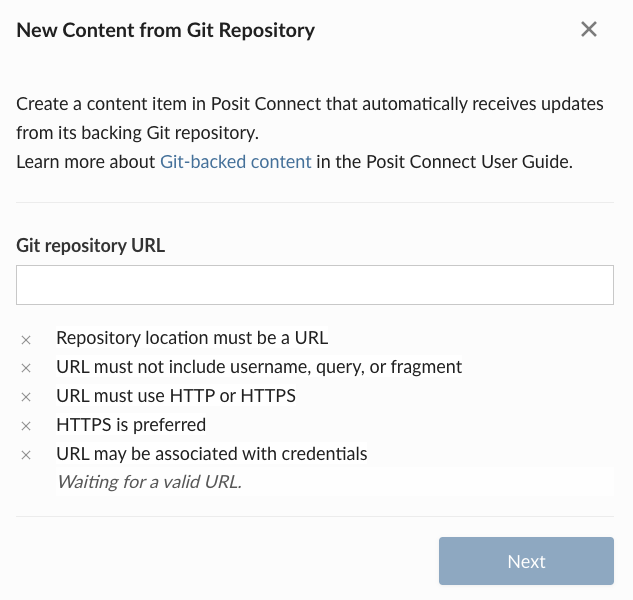
\includegraphics[width=4.5in,height=\textheight]{images/repo-url.png}

}

\caption{\label{fig-repo-url}Git Repository URL}

\end{figure}%

After supplying the URL, click \textbf{Next} where you'll be asked to
select a branch. This repository only contains a single branch called
\texttt{main}. Ensure \texttt{main} is selected and click \textbf{Next}.

\begin{tcolorbox}[enhanced jigsaw, toprule=.15mm, title=\textcolor{quarto-callout-tip-color}{\faLightbulb}\hspace{0.5em}{Tip}, opacitybacktitle=0.6, titlerule=0mm, arc=.35mm, bottomrule=.15mm, rightrule=.15mm, colbacktitle=quarto-callout-tip-color!10!white, coltitle=black, colframe=quarto-callout-tip-color-frame, left=2mm, opacityback=0, colback=white, breakable, bottomtitle=1mm, toptitle=1mm, leftrule=.75mm]

You can deploy the same piece of content from a single git repository!
For example, maybe you have a developmental version on a \texttt{dev}
branch, and a production version on the \texttt{main} branch.

\end{tcolorbox}

\section{Step 3 - Deploy Content}\label{step-3---deploy-content}

At this point, Posit Connect will look for ``deployable directories.''
In other words, it's looking for directories in the repository that
contain a \texttt{manifest.json} file. There should only be one
deployable directory (\texttt{shiny-app-r}). Ensure it's selected, give
your application a name, then click \textbf{Deploy Content}!

\begin{figure}

\centering{

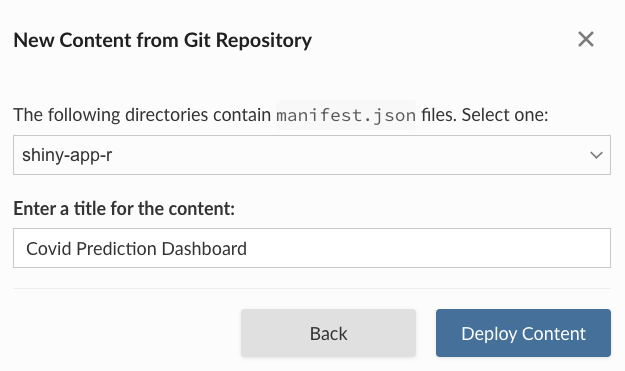
\includegraphics[width=4.70833in,height=\textheight]{images/deploy-content.png}

}

\caption{\label{fig-deploy-content}Deploy Content from Git Repository}

\end{figure}%

Connect will then read the \texttt{manifest.json} file and install any
environment dependencies needed to ensure the application runs properly.
After the deployment process is complete, click \textbf{Open Content} to
view the application on Posit Connect!

\begin{figure}

\centering{

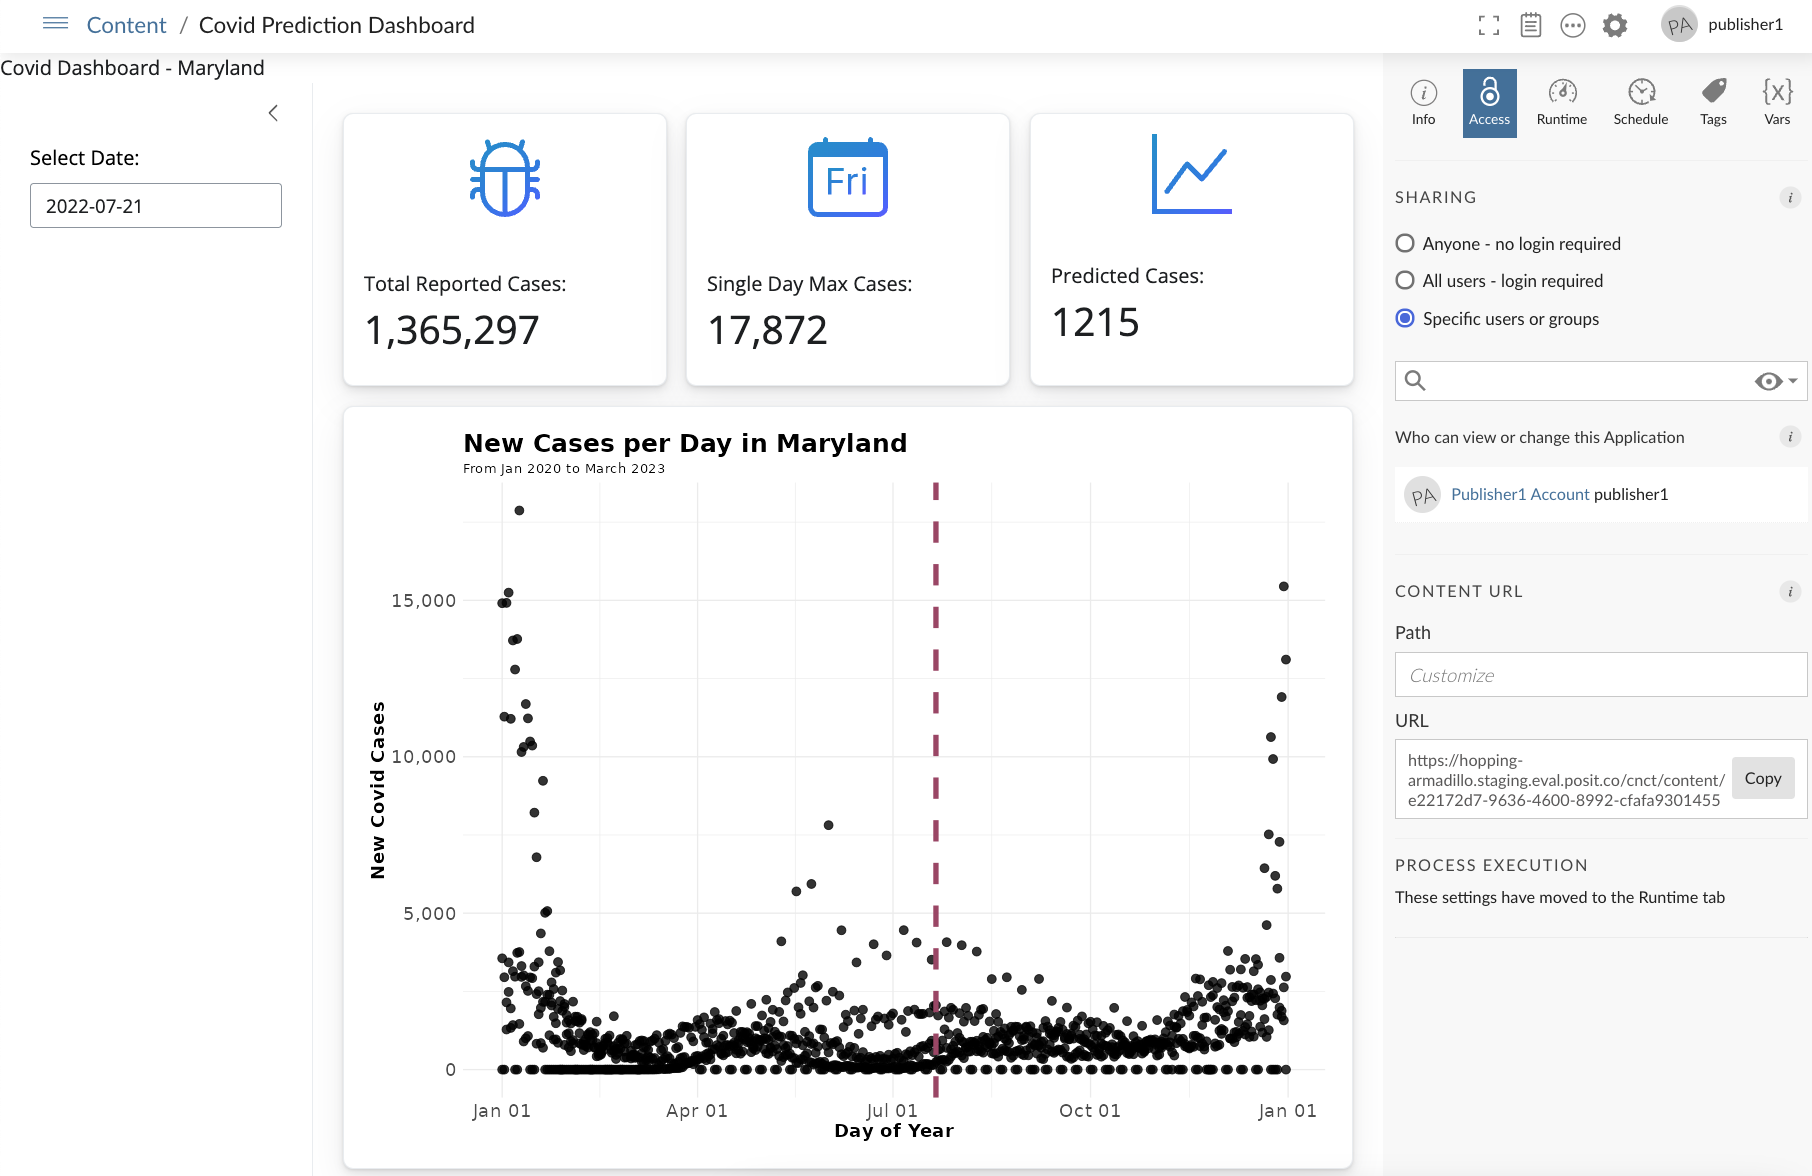
\includegraphics{images/covid-dashbaord.png}

}

\caption{\label{fig-covid-dashboard}Covid Dashboard}

\end{figure}%

This shiny dashboard tells us the same information as our previous shiny
for Python application: how many new COVID cases are predicted for a
given day of the year. As you can see, this application has some
additional details and features that greatly improve the user experience
including the total number of COVID cases for the given state/province,
and the single day max number of new COVID cases.

By default, Posit Connect will scan the linked git repository for any
changes every 15 minutes. If any changes were detected (e.g., a new
commit to the \texttt{main} branch), Posit Connect will automatically
redeploy the application! You can also manually check for repository
updates by clicking the \textbf{Info} tab in the top right corner and
selection \textbf{Update Now} from the side bar:

\begin{figure}

\centering{


\includegraphics{images/update-content.png}

}

\caption{\label{fig-update-content}Manually Check Git Repository for
Changes}

\end{figure}%

\part{Bonus Content}

\chapter{Bonus Content}\label{bonus-content-1}



\end{document}
